\documentclass{beamer}
\mode<presentation>
\usepackage[utf8]{inputenc}
\usepackage{algorithm,algorithmicx,amssymb,amsmath,amsthm,bbm,color,epstopdf,float,geometry,graphicx,hyperref,listings,mathrsfs,mathtools,multirow,subcaption,textgreek,xcolor}

\usepackage[noend]{algpseudocode}
\usepackage{algcompatible}



\usepackage{float}
\renewcommand{\algorithmicrequire}{\textbf{Input:}}
\renewcommand{\algorithmicensure}{\textbf{Output:}}
    
% \usepackage[linesnumbered,ruled,vlined]{algorithm2e}
\usepackage[flushleft]{threeparttable}
\usepackage[shortlabels]{enumitem}
\usepackage[table]{xcolor}
\newcommand{\JLcolor}[1]{{\textcolor{violet}{#1}}} %violet

% Create Background Pic
%\usepackage{tikz}
%\definecolor{bottomcolour}{rgb}{0.32,0.3,0.38}
%\definecolor{topcolour}{rgb}{0.08,0.08,0.16}
%\setbeamertemplate{background canvas}{%
%	\begin{tikzpicture}[remember picture,overlay]
%	\shade[top color=topcolour,bottom color=bottomcolour]
%(current page.north west) rectangle (current page.south east);
%	\end{tikzpicture}%     
%}


%=======================================================
% Set page number
\setbeamertemplate{footline}[page number]

%=======================================================
%\usetheme{Boadilla}
\setbeamerfont{title}{size=\fontsize{18pt}{18pt}\selectfont} % bold font: \bfseries
\setbeamerfont{author}{size=\fontsize{20pt}{20pt}\selectfont}
\setbeamerfont{institute}{size=\fontsize{13pt}{13pt}\selectfont}
%\setbeamercolor{itemize item}{fg=red}

%================================================
%Set font color
\definecolor{mygray1}{rgb}{0.7421875,0.7421875,0.7421875}
\definecolor{mygray2}{gray}{0.6}
\definecolor{mygray3}{rgb}{0.55, 0.52, 0.54}
\definecolor{mybrown1}{rgb}{0.28, 0.24, 0.2}
\definecolor{myred}{rgb}{0.68, 0.09, 0.13}
\definecolor{myginger}{rgb}{0.69, 0.4, 0.0}
\definecolor{myblue1}{rgb}{0.0, 0.2, 0.6}
\definecolor{myblue2}{rgb}{0.38, 0.51, 0.71}
\definecolor{myblue3}{rgb}{0.2,0.2,0.7}
\definecolor{mygreen}{rgb}{0.42, 0.56, 0.14}
\definecolor{myviolet}{rgb}{0.54, 0.17, 0.89}


\newcommand{\highlightA}[1]{\colorbox{myblue3!50!}{$\displaystyle #1$}}
\newcommand{\highlightB}[1]{\colorbox{myred!50!}{$\displaystyle #1$}}
\newcommand{\highlightC}[1]{\colorbox{mygreen!50!}{$\displaystyle #1$}}
%================================================
% set picture source
\usepackage[absolute,overlay]{textpos}

\setbeamercolor{framesource}{fg=gray}
\setbeamerfont{framesource}{size=\tiny}
\newcommand{\source}[1]{\begin{textblock*}{4cm}(8.7cm,8.6cm)
\begin{beamercolorbox}[ht=0.5cm,right]{framesource}
\usebeamerfont{framesource}\usebeamercolor[fg]{framesource} Source: {#1}
\end{beamercolorbox}
\end{textblock*}}

\setbeamercolor{frametitle}{fg=white,bg=black}


%================================================
% url color
\renewcommand\UrlFont{\color{myblue3}}
%================================================

\newtheorem{Thm}{{\bf Theorem}}


% Make first page
\makeatletter
\setbeamertemplate{navigation symbols}{}
\title[MFMC for Tokamak UQ]{Multi-fidelity Monte Carlo for Uncertainty Quantification in the Free-Boundary Grad–Shafranov Equation}
%\subtitle[short version]{}
%\date{}
\author[J.Liang]{\normalsize  Jiaxing Liang\\ Matthias Heinkenschloss}
\institute[Rice University]{\fontsize{8}{8} Department of Computational and Applied Mathematics, Rice University}




%=======================================================
\begin{document}
\frame{\titlepage }

%------------------------------------------------------------
% {\setbeamertemplate{footline}{} 
\begin{frame}[c]		
\frametitle{Outline}
\normalsize
\begin{itemize}[leftmargin=5pt] 
\item[$\triangleright$] Physical Model: Grad-Shafranov Equation
\vspace{0.3cm}
\item[$\triangleright$] Uncertainty Quantification 
\vspace{0.3cm}
\item[$\triangleright$] Objectives \& Approaches
% \vspace{0.3cm}
% \item[$\triangleright$] Surrogate via Sparse Grid Stochastic Collocation
\vspace{0.3cm}
\item[$\triangleright$] Multi-fidelity Monte Carlo
\vspace{0.3cm}
\item[$\triangleright$] Parameter Estimation
\vspace{0.3cm}
\item[$\triangleright$] Numerical Results
\end{itemize}
\end{frame}
% }


%------------------------------------------------------------
% \addtocounter{page}{-1}
\begin{frame}[noframenumbering]
\setbeamercolor{itemize item}{fg=mygray1}
\large 	
\textcolor{mygray1}{
    \begin{itemize}[leftmargin=5pt] 
        \item[\textcolor{black}{$\triangleright$}] \textcolor{black}{\fontsize{25}{60}\selectfont Physical Model: Grad-Shafranov Equation}
        \vspace{0.2cm}	
        \item[$\triangleright$] Uncertainty Quantification
        \vspace{0.2cm}
        \item[$\triangleright$] Objectives \& Approaches
        \vspace{0.2cm}
        \item[$\triangleright$] Multi-fidelity Monte Carlo
            % \vspace{0.3cm}
            % {\footnotesize
            % \begin{itemize}[leftmargin=15pt]   
            %     \item[$\circ$] Surrogate via Sparse Grid Stochastic Collocation
            %     % \vspace{0.3cm}
            %     \item[$\circ$] Experimental Results \& Conclusions
            % \end{itemize}
            % }
        \vspace{0.2cm}
        \item[$\triangleright$] Parameter Estimation
            % \vspace{0.3cm}
            % {\footnotesize
            % \begin{itemize}[leftmargin=15pt]   
            %     \item[$\circ$] Monte Carlo \& Uniform Multilevel Monte Carlo
            %     \item[$\circ$] Adaptive Multilevel Monte Carlo
            %     \item[$\circ$] Experimental Results \& Conclusions
            % \end{itemize}
            % }
        \vspace{0.2cm}
        \item[$\triangleright$] Numerical Results
            % {\footnotesize
            % \begin{itemize}[leftmargin=15pt]   
            %     \item[$\circ$] Three Types of Surrogates
            %     \item[$\circ$] Surrogate-based Samplings
            %     \item[$\circ$] Experimental Results \& Conclusions
            % \end{itemize}
            % }
        % \vspace{0.2cm}
        % \item[$\triangleright$] Approach 4: Multi-fidelity Monte Carlo
    \end{itemize}
}
\end{frame}
%------------------------------------------------------------



\begin{frame}[t]{stellar}
\frametitle{Fusion \& Magnetic Confinement}
{\footnotesize
\begin{itemize}[leftmargin=5pt] 
    \item[$\triangleright$]  \textcolor{myblue3}{\bf \normalsize Fusion reactor:} Focus on Tokamak -- doughnut-shaped vacuum chamber. 
    
    \item[$\triangleright$] \textcolor{myblue3}{\bf\normalsize  Fusion mechanism:} Inject fuel gas (hydrogen isotopes) into the chamber $\rightarrow$ heated with microwave $\rightarrow$ form a plasma $\rightarrow$ particles overcome coulomb repulsion $\rightarrow$ fuse to produce energy.
    
    \vspace{0.1cm}
    \begin{figure}[H]	
    \centering
    \begin{tabular}{ccc}
    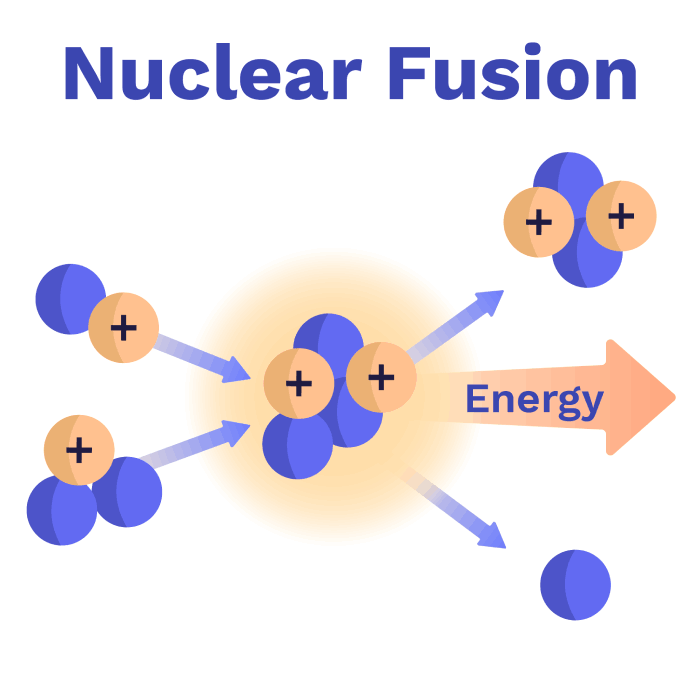
\includegraphics[height=0.2\linewidth]{./figures_slides/fusion_reaction.png}&\qquad \qquad
    \includegraphics[height=0.2\linewidth]{./figures_slides/ITER}&
    % \includegraphics[height=0.26\linewidth]{"IterChamber"}
    \end{tabular}
    \source{https://www.iter.org/mach/Tokamak}
    \end{figure}

        \item[$\triangleright$] During fusion, the hot plasma tends to expand, to prevent it from contacting the reactor wall, it must be confined. 
        \item[$\triangleright$] \textcolor{myblue3}{\bf\normalsize  Magnetic confinement:} Confinement is achieved through magnetic fields generated by currents running through external coils surrounding the reactor.
        \item[$\triangleright$] Our project focuses on studying the \textcolor{myred}{\bf impact of variations in current} on the physical properties of the confinement field. These \textcolor{myred}{\bf variations} may come from power supply, temperature fluctuations, and material impurities in the conduction wire.
\end{itemize}
}	
\end{frame}




%------------------------------------------------------------
\begin{frame}[t]
\frametitle{The Grad-Shafranov Free Boundary Problem}
\vspace{-4mm}
\begin{minipage}[t]{\linewidth}
    {\footnotesize
        \begin{subequations}
            \begin{equation*}
            -\nabla\,\cdot\,\left(\frac{1}{\mu x}\nabla\psi\right) = \left\{ \begin{array}{ll}
            x\frac{d}{d\psi} p(\psi) + \frac{1}{2\, \mu x} \frac{d}{d\psi}  g^2(\psi) & \text{ in } \underline{\Omega_p(\psi)} \\
            \boldsymbol{I_i}/S_i & \text{ in } \Omega_{C_i} \\
            0 & \text{ elsewhere } 
            \end{array}\right.
            \end{equation*}
            \begin{equation*}
            \psi(0,y) = 0 ; \qquad \qquad  \lim_{\|(x,y)\|\to\infty}\psi(x,y) = 0. 
            \end{equation*}
        \end{subequations}}

{\footnotesize
              \begin{itemize}[leftmargin=0pt] 
                    \item[]	\textcolor{myblue3}{$\psi$:} \textcolor{mybrown1}{poloidal flux.}
                    \; \textcolor{myblue3}{$\mu(\psi)$:} \textcolor{mybrown1}{magnetic permeability.} 
                    \; \textcolor{myblue3}{$p(\psi)$:} \textcolor{mybrown1}{hydrodynamic pressure}.
                    
                    \vspace{-1.5mm}
                    \item[]	\textcolor{myblue3}{$g(\psi)$:}  \textcolor{mybrown1}{toroidal field function.}
                    \;\textcolor{myblue3}{$\Omega_p(\psi)$:} \textcolor{mybrown1}{confinement region.}
                    \;\textcolor{myblue3}{$I_i$:} \textcolor{mybrown1}{current intensity.}

                    \vspace{-1.5mm}
                    \item[]	\textcolor{myblue3}{$S_i$:} \textcolor{mybrown1}{cross section area of the coils.}\quad \textcolor{myblue3}{$\Omega_{c_i}$:} \textcolor{mybrown1}{locations of coils.}
                \end{itemize}
    }
    
    \begin{columns}
        %	\hspace{-3mm}
        \begin{column}{0.66\linewidth}
            {\small
                % \begin{itemize}[leftmargin=5pt] 
                %     \item[]	\textcolor{myblue3}{$\psi$:} \textcolor{mybrown1}{poloidal flux function.}
                %     \vspace{-1.5mm}
                %     %			\vspace{-5mm}
                %     \item[]	\textcolor{myblue3}{$p(\psi)$:} \textcolor{mybrown1}{hydrodynamic pressure}.
                %     \vspace{-1.5mm}
                %     %		\vspace{-4mm}
                %     \item[]	\textcolor{myblue3}{$I_i$:} \textcolor{mybrown1}{current intensity in the coils.}
                %     \vspace{-1.5mm}
                %     \item[]	\textcolor{myblue3}{$\Omega_p(\psi)$:} \textcolor{mybrown1}{confinement region.}
                %     \vspace{-1.5mm}
                %     \item[]	\textcolor{myblue3}{$\mu(\psi)$:} \textcolor{mybrown1}{magnetic permeability.}
                %     \vspace{-1.5mm} 
                %     \item[]	\textcolor{myblue3}{$g(\psi)$:}  \textcolor{mybrown1}{toroidal field function.}
                %     \vspace{-1.5mm}
                %     \item[]	\textcolor{myblue3}{$S_i$:} \textcolor{mybrown1}{cross section area of the coils.}
                %     \vspace{-1.5mm}
                %     \item[]	\textcolor{myblue3}{$\Omega_{c_i}$:} \textcolor{mybrown1}{locations of coils.}
                % \end{itemize}
            \vspace{-3mm}
            \begin{itemize}[leftmargin=40pt] 
            % \item[$\circ$] Physical space: 2-d.
            % \item[$\circ$] {\bf Knowns:} $ p(\psi), g(\psi), I_i, \Omega_{c_i}$, and  $\mu$. {\bf Unknowns:} $\psi$ and $\Omega_p(\psi)$.

            \item[$\circ$] {\bf Non-linear} \underline{free boundary problem} with the source of uncertainty arises from the \textcolor{myred}{\bf current intensities}.

            \item[$\circ$] {\bf Knowns:} $ p(\psi), g(\psi), I_i, \Omega_{c_i}$, and  $\mu$. {\bf Unknowns:} $\psi$ and $\Omega_p(\psi)$.
            
            \item[$\circ$] \textcolor{myblue3}{\bf Software:} \textsc{Matlab} finite element package {\tt FEEQS.M} -- H. Heumann and his collaborators.

        %     {\fontsize{7.5}{7.5}\selectfont \textcolor{mygray2}{
        % H. Heumann, J. Blum, C. Boulbe, B. Faugeras, G. Selig, J.-M. Ané, S. Brémond, V. Grandgirard, P. Hertout, E. Nardon, et al., Quasi-static free-boundary
        %     equilibrium of toroidal plasma with CEDRES: computational methods and applications, J. Plasma Phys. 81 (3) (2015) 905810301.}\par}
            \end{itemize}
            }
        \end{column}
        
        % \hspace{-3mm}
        \begin{column}{0.5\linewidth}
        \vspace{-6mm}
            \begin{figure}[H]	
                \centering
                \hspace{-17mm}
                \begin{tabular}{cc}
                    \begin{subfigure}{0.5\textwidth}
                    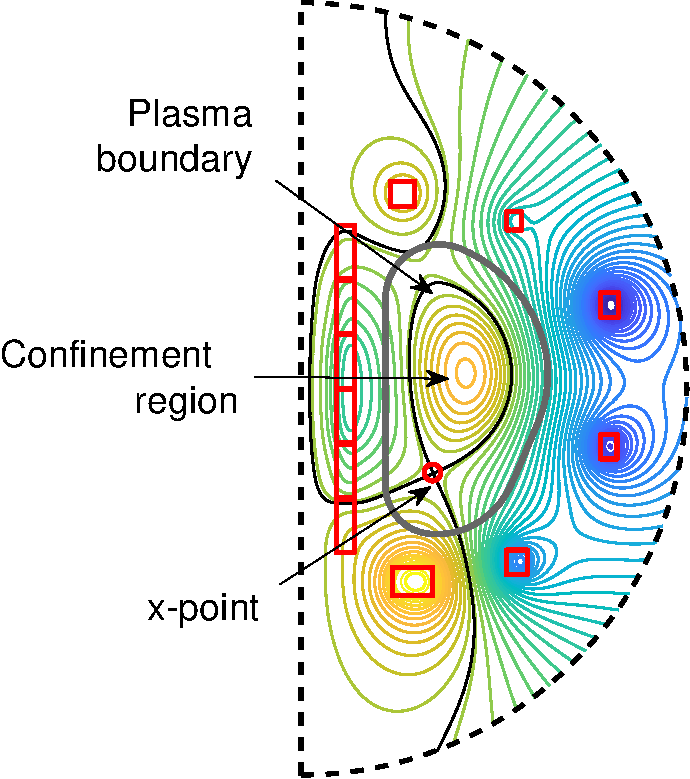
\includegraphics[height=1.8\linewidth]{./figures_slides/FreeBoundary_contoursWstructures}
                        %					\caption*{Diverted configuration}
                    \end{subfigure}
                \end{tabular}
            \end{figure}
        \end{column}
    \end{columns}
\end{minipage}
\end{frame}



%------------------------------------------------------------
\begin{frame}[c]
\setbeamercolor{itemize item}{fg=mygray1}
\large 	
\textcolor{mygray1}{
    \begin{itemize}[leftmargin=5pt] 
        \item[$\triangleright$]  Physical Model: Grad-Shafranov Equation
        \vspace{0.2cm}	
        \item[\textcolor{black}{$\triangleright$}] \textcolor{black}{\fontsize{25}{60}\selectfont Uncertainty Quantification}
        \vspace{0.2cm}
        \item[$\triangleright$] Objectives \& Approaches
        \vspace{0.2cm}
        \item[$\triangleright$] Multi-fidelity Monte Carlo
            % \vspace{0.3cm}
            % {\footnotesize
            % \begin{itemize}[leftmargin=15pt]   
            %     \item[$\circ$] Surrogate via Sparse Grid Stochastic Collocation
            %     % \vspace{0.3cm}
            %     \item[$\circ$] Experimental Results \& Conclusions
            % \end{itemize}
            % }
        \vspace{0.2cm}
        \item[$\triangleright$] Parameter Estimation
            % \vspace{0.3cm}
            % {\footnotesize
            % \begin{itemize}[leftmargin=15pt]   
            %     \item[$\circ$] Monte Carlo \& Uniform Multilevel Monte Carlo
            %     \item[$\circ$] Adaptive Multilevel Monte Carlo
            %     \item[$\circ$] Experimental Results \& Conclusions
            % \end{itemize}
            % }
        \vspace{0.2cm}
        \item[$\triangleright$] Numerical Results
            % {\footnotesize
            % \begin{itemize}[leftmargin=15pt]   
            %     \item[$\circ$] Three Types of Surrogates
            %     \item[$\circ$] Surrogate-based Samplings
            %     \item[$\circ$] Experimental Results \& Conclusions
            % \end{itemize}
            % }
        % \vspace{0.2cm}
        % \item[$\triangleright$] Approach 4: Multi-fidelity Monte Carlo
    \end{itemize}
}
\end{frame}


%------------------------------------------------------------
\begin{frame}[t]
    \frametitle{Uncertain Coil Currents}
    \begin{itemize}[leftmargin=5pt]
        \item[$\triangleright$] \textcolor{myblue3}{\bf Source of uncertainty:} {\footnotesize Investigate the impact of \textcolor{myblue3}{uncertainties in the current intensities} on the confinement properties of a plasma.}
        
        \item[$\triangleright$] \textcolor{myred}{\bf Baseline current intensities:} 
        \[
        \footnotesize
        \begin{array}{lll}
        I_1: -1.40\times 10^6\text{A} &I_5: -9.00\times 10^6\text{A} &I_9:  -6.43\times 10^6\text{A} \\
        I_2: -9.50\times 10^6\text{A} &I_6: 3.56\times 10^6\text{A}  & I_{10}:  -4.82\times 10^6\text{A} \\
        I_3: -2.04\times 10^7\text{A} &I_7:  5.47\times 10^6\text{A}  &I_{11}:  -7.50\times 10^6\text{A} \\
        I_4: -2.04\times 10^7\text{A} &I_8: -2.27\times 10^6\text{A} &I_{12}:  1.72\times 10^7\text{A} 
        \end{array}
        \]
        \item[$\triangleright$] \textcolor{myblue3}{\bf Uncertianty Quantification (UQ):} {\footnotesize Variations in the baseline current intensities. Each current in the array is considered to be a parameter, so we have 12-dimensional parameter space.}
        
        
        \item[$\triangleright$] \textcolor{myblue3}{\bf Currents uniformly distributed:} 

        {\footnotesize
        \textcolor{mygray3}{$\tau$: perturbation level ($\tau= 1\%$ \& $2\%$). \quad $I_k$: current intensity in the $k$-th coil.}
        

        \begin{itemize}[leftmargin=15pt]   
            \item[$\circ$] Joint density function: $\displaystyle
             \pi \left(\boldsymbol{\omega}\right)=\prod_{k=1}^{d} \pi_k\left(\omega_{k}\right)=\prod_{k=1}^{d} \frac{1}{2\tau |I_k|}$.
            \item[$\circ$] 12-d parameter space: $\displaystyle W := \prod_{k=1}^{d}\left[I_k-\tau|I_k|,I_k+\tau|I_k|\right]$.
        \end{itemize}
        \par}
    \end{itemize}
\end{frame}	

%------------------------------------------------------------
\begin{frame}[c]
\setbeamercolor{itemize item}{fg=mygray1}
\large 	
\textcolor{mygray1}{
    \begin{itemize}[leftmargin=5pt] 
        \item[$\triangleright$]  Physical Model: Grad-Shafranov Equation
        \vspace{0.2cm}	
        \item[$\triangleright$] Uncertainty Quantification
        \vspace{0.2cm}
        \item[\textcolor{black}{$\triangleright$}] \textcolor{black}{\fontsize{25}{60}\selectfont Objectives \& Approaches}
        \vspace{0.2cm}
        \item[$\triangleright$] Multi-fidelity Monte Carlo
            % \vspace{0.3cm}
            % {\footnotesize
            % \begin{itemize}[leftmargin=15pt]   
            %     \item[$\circ$] Surrogate via Sparse Grid Stochastic Collocation
            %     % \vspace{0.3cm}
            %     \item[$\circ$] Experimental Results \& Conclusions
            % \end{itemize}
            % }
        \vspace{0.2cm}
        \item[$\triangleright$] Parameter Estimation
            % \vspace{0.3cm}
            % {\footnotesize
            % \begin{itemize}[leftmargin=15pt]   
            %     \item[$\circ$] Monte Carlo \& Uniform Multilevel Monte Carlo
            %     \item[$\circ$] Adaptive Multilevel Monte Carlo
            %     \item[$\circ$] Experimental Results \& Conclusions
            % \end{itemize}
            % }
        \vspace{0.2cm}
        \item[$\triangleright$] Numerical Results
            % {\footnotesize
            % \begin{itemize}[leftmargin=15pt]   
            %     \item[$\circ$] Three Types of Surrogates
            %     \item[$\circ$] Surrogate-based Samplings
            %     \item[$\circ$] Experimental Results \& Conclusions
            % \end{itemize}
            % }
        % \vspace{0.2cm}
        % \item[$\triangleright$] Approach 4: Multi-fidelity Monte Carlo
    \end{itemize}
}
\end{frame}
%------------------------------------------------------------



%------------------------------------------------------------
\begin{frame}[t]
    \frametitle{Objectives \& approaches}
        \begin{itemize}[leftmargin=5pt] 
            
            \item[$\triangleright$] \textcolor{myblue3}{\bf Uncertainty Quantification in Plasma Equilibria} 
            
            {\fontsize{9}{9}\selectfont
            Quantify the {\bf impact of variations in current intensity} on determining 
            \begin{itemize}[leftmargin=15pt]     
                \item[\textcolor{myblue3}{$\bullet$}]   {\bf Expectation:}
                $\mathbb{E}\left[\psi(x,y,\boldsymbol \omega)\right]=\int_W \psi(x,y,\boldsymbol{\omega})\pi(\boldsymbol\omega)d\boldsymbol{\omega}.$
            
                \vspace{0.5mm}
                \item[\textcolor{myblue3}{$\bullet$}] {\bf Key plasma features:}  presence and locations of x-points, contact points, strike points \& separatrices.
                %the location where the poloidal flux function achieves saddle point
                % \item[$\circ$] \textcolor{mygray2}{Presence of strike points \& contact points.}\\

                \vspace{0.5mm}
                \item[\textcolor{myblue3}{$\bullet$}]  {\bf Geometry parameters:} elongation, triangularity etc.
                
                %						\text {Geometric parameters}
                % determint the most likely location of strike points
                % standard deviation
                %the location where the poloidal flux function achieves maximum or minimum
            \end{itemize}
            }
            \vspace{2mm}
            \item[$\triangleright$] \textcolor{myblue3}{\bf Enhancing Sampling Efficiency}
            
            {\fontsize{9}{9}\selectfont
            Use {\bf sampling methods} to approximate the expectation efficiently
            \begin{itemize}[leftmargin=15pt] 
                \item[\textcolor{myblue3}{$\bullet$}] \textcolor{myblue3}{Multi-fidelity Monte Carlo}
                
                \textcolor{mybrown1}{{\bf Blending high- and low-fidelity models}, where high-fidelity models provide accuracy and low-fidelity surrogates reduce computational cost.}

                
                % \vspace{2mm}
                % \item[\textcolor{myblue3}{$\bullet$}] \textcolor{myblue3}{Approach 1: Surrogate-based Monte Carlo}
                
                % \textcolor{mybrown1}{Replace the nonlinear solution with a {\bf surrogate function} for Monte Carlo sampling.}

                % \vspace{2mm}
                % \item[\textcolor{myblue3}{$\bullet$}] \textcolor{myblue3}{Approach 2: Multilevel Monte Carlo}
                
                % \textcolor{mybrown1}{Improve efficiency by using another sampling approach -- {\bf multilevel Monte Carlo method}.}

                % \vspace{2mm}
                % \item[\textcolor{myblue3}{$\bullet$}] \textcolor{myblue3}{Numerical Results}
                
                % \textcolor{mybrown1}{Further improve efficiency by using a {\bf hybrid method} that combines surrogate and multilevel Monte Carlo. }
        
            \end{itemize}
            }
            \vspace{2mm}
            \item[$\triangleright$] \textcolor{myblue3}{\bf New Contributions}
                {\fontsize{9}{9}\selectfont
                \begin{itemize}[leftmargin=15pt] 
                \item[\textcolor{myblue3}{$\bullet$}] Optimization-based formulation for MFMC sample allocation.
                \item[\textcolor{myblue3}{$\bullet$}] Dynamic pilot sampling strategy for correlation estimation.
                \end{itemize}
                }
    \end{itemize}
\end{frame}


%------------------------------------------------------------
\begin{frame}[c]
\setbeamercolor{itemize item}{fg=mygray1}
\large 	
\textcolor{mygray1}{
    \begin{itemize}[leftmargin=5pt] 
        \item[$\triangleright$]  Physical Model: Grad-Shafranov Equation
        \vspace{0.2cm}	
        \item[$\triangleright$] Uncertainty Quantification
        \vspace{0.2cm}
        \item[$\triangleright$]  Objectives \& Approaches
        \vspace{0.2cm}
        \item[\textcolor{black}{$\triangleright$}] \textcolor{black}{\fontsize{25}{60}\selectfont Multi-fidelity Monte Carlo}
            % \vspace{0.3cm}
            % {\footnotesize
            % \begin{itemize}[leftmargin=15pt]   
            %     \item[$\circ$] Surrogate via Sparse Grid Stochastic Collocation
            %     % \vspace{0.3cm}
            %     \item[$\circ$] Experimental Results \& Conclusions
            % \end{itemize}
            % }
        \vspace{0.2cm}
        \item[$\triangleright$] Parameter Estimation
            % \vspace{0.3cm}
            % {\footnotesize
            % \begin{itemize}[leftmargin=15pt]   
            %     \item[$\circ$] Monte Carlo \& Uniform Multilevel Monte Carlo
            %     \item[$\circ$] Adaptive Multilevel Monte Carlo
            %     \item[$\circ$] Experimental Results \& Conclusions
            % \end{itemize}
            % }
        \vspace{0.2cm}
        \item[$\triangleright$] Numerical Results
            % {\footnotesize
            % \begin{itemize}[leftmargin=15pt]   
            %     \item[$\circ$] Three Types of Surrogates
            %     \item[$\circ$] Surrogate-based Samplings
            %     \item[$\circ$] Experimental Results \& Conclusions
            % \end{itemize}
            % }
        % \vspace{0.2cm}
        % \item[$\triangleright$] Approach 4: Multi-fidelity Monte Carlo
    \end{itemize}
}
\end{frame}
%------------------------------------------------------------


%------------------------------------------------------------
\begin{frame}[t]
\frametitle{Monte Carlo Sampling}

\begin{itemize}[leftmargin=5pt] 
    \item[$\triangleright$] \textcolor{myblue3}{\bf Monte Carlo sampling (MC)}
    
    {\footnotesize 
    Estimate $\mathbb{E}[u]$ by  a finite number of i.i.d. sample average.
        \[
    A^{\text{MC}}_N:= \frac {1}{N}\sum_{i=1}^N u_h^{(i)}.
    \vspace{-2mm}
    \]
     }       
    \item[$\triangleright$] \textcolor{myblue3}{\bf MC estimator $A^{\text{MC}}$ for $\mathbb{E}[u]$}
    {\footnotesize 
    \begin{itemize}[leftmargin=15pt] 
    \item[$\circ$] Unbiased $\mathbb{E}[A^{\text{MC}}_N] = \mathbb{E}[u_h]$.
    \item[$\circ$] Variance decays slowly: $\mathcal{O}(N^{-1/2})$. $\mathbb{V}[A^{\text{MC}}_N]= \mathbb{V}[u_h]/N$, where $
    \mathbb{V}[u_h] = \frac{1}{N-1}\left(\sum_{i=1}^{N}\left\Vert u_h^{(i)}\right\Vert_{U}^2-\frac{1}{N}\left\Vert\sum_{i=1}^{N}u_h^{(i)}\right\Vert_{U}^2\right).
    $
    \end{itemize}
    }
    % \vspace{2mm}
    % $u$: Solution of PDE. 
    
    % $u_{h}$: Approximation of $u$ based on discretization parameter $h$. 
    
    % $u_h^{(i)} = u_h(\omega^{(i)})$: realization of the $i$-th random sample $\omega^{(i)}$. 	 
    
    % $N$: Number of samples. 
            
\end{itemize}

\end{frame}


%------------------------------------------------------------
\begin{frame}[t]
    \frametitle{Multi-fidelity Monte Carlo}
\begin{itemize}[leftmargin=5pt] 
\item[$\triangleright$] \textcolor{myblue3}{\bf Multi-fidelity Monte Carlo (MFMC)} 

{\footnotesize A variance reduction technique that efficiently estimates statistical quantities by using low fidelity (LF) models to reduce variance of high fidelity (HF) model. HF models are used to maintaining accuracy.}

%
\vspace{2mm}
%
{\fontsize{7}{7}\selectfont \textcolor{mygray2}{B. Peherstorfer, K. Willcox, and M. Gunzburger. Optimal Model Management for Multifidelity Monte Carlo Estimation. SIAM J. SCI. COMPUT, Vol. 38, No. 5, pp. A3163–A3194.}\par}
%

\item[$\triangleright$]\textcolor{myblue3}{\bf MFMC estimator $A^{\text{MF}}$ for $\mathbb{E}[u]$} 

{\footnotesize 
\vspace{-3mm}
\begin{align*}
A^{\text{MF}} &= A^{\text{MC}}_{1,N_1} + \sum_{k=2}^K \alpha_k\left(\overline{A}_{k,N_k} - \overline{A}_{k,N_{k-1}} \right)
    % &= A^{\text{MC}}_{1,N_1} +  \sum_{k=2}^K \alpha_k\left(\frac{N_{k-1}}{N_{k}}-1\right)\left(A_{k,N_{k-1}}^{\text{MC}}- A_{k,N_k\backslash N_{k-1}}^{\text{MC}}\right) 
\end{align*}
\vspace{-3mm}

\begin{itemize}[leftmargin=15pt] 
    \item[$\circ$] $\overline{A}_{k,N_{k-1}}$ reuses the first $N_{k-1}$ samples from $\overline{A}_{k,N_{k}}$, $N_k\ge N_{k-1}$.
    \item[$\circ$] Unbiased $\mathbb{E}[A^{\text{MF}}] = \mathbb{E}[u_h]$.
    \item[$\circ$] Let $\Delta_k = \rho_{1,k}^2 - \rho_{1,k+1}^2$ for $k = 1, \dots, K$, with $\rho_{1,K+1} = 0$, $\mathbb{V}[A^{\text{MF}}]= \sigma_1^2\sum_{k=1}^K\frac{\Delta_{k}}{N_k}$.
    \item[$\circ$] Requires estimating optimal weights $\alpha_k$ and sample sizes $N_k$.
    \item[$\circ$] Efficiency depends on correlation $\rho_{1,k}$ between HF and LF.
\end{itemize}
}
\end{itemize}
\end{frame}


%------------------------------------------------------------
\begin{frame}[t]
    \frametitle{Multi-fidelity Monte Carlo}
\begin{itemize}[leftmargin=5pt] 
\item[$\triangleright$] \textcolor{myblue3}{\bf HF and LF models} 

{\footnotesize 
\begin{itemize}[leftmargin=5pt] 
     \item[$\circ$] {\bf High fidelity models:} Expensive but accurate 
     
     (e.g., finite element solution of Grad-Shafranov equation).
     \item[$\circ$] {\bf Low fidelity models:} Cheap but less accurate, correlated with HF as control variates.
     
     (e.g., sparse grid stochastic collocation $+$ coarser meshes).


\end{itemize}
 }
% \item[$\triangleright$] \textcolor{myblue3}{\bf Offline cost} 

% {\footnotesize 
% Construction of low fidelity models, parameter estimation, model selection.
% }
\end{itemize}
\end{frame}

% %------------------------------------------------------------
\begin{frame}[t]
    \frametitle{Sparse Grid Stochastic Collocation}
\begin{itemize}[leftmargin=5pt] 

\item[$\triangleright$] Build surrogate via \textcolor{myblue3}{\bf Sparse Grid Stochastic Collocation}.
\vspace{2mm}
    \begin{itemize}[leftmargin=7pt] 
        \item [$\circ$] {\bf Idea:} {\footnotesize Select a special set of current  $\{\boldsymbol{\omega}^{(k)}\}_{1 \le k\le n_{sc}}$ in the parameter space. For each $\boldsymbol{\omega}^{(k)}$, evaluate the nonlinear solver to yield the realization $\{\psi_h^{(k)}\}$. An interpolation (surrogate) is then constructed to mimic the original nonlinear function with 
        \vspace{-3mm}
        $$\hspace{15mm}\widehat{\psi_h}(\cdot, \boldsymbol{\omega}) = \sum_k\psi_h^{(k)}(\cdot)L_{\boldsymbol{\omega}^{(k)}}(\boldsymbol{\omega}).$$
        \par}
    
        \vspace{2mm}
        \item [$\circ$] {\bf Sparse grids}: 
        \vspace{-8mm}
        \begin{figure}[H]	
        \centering
        \hspace{19mm}
        \begin{tabular}{ccc}
            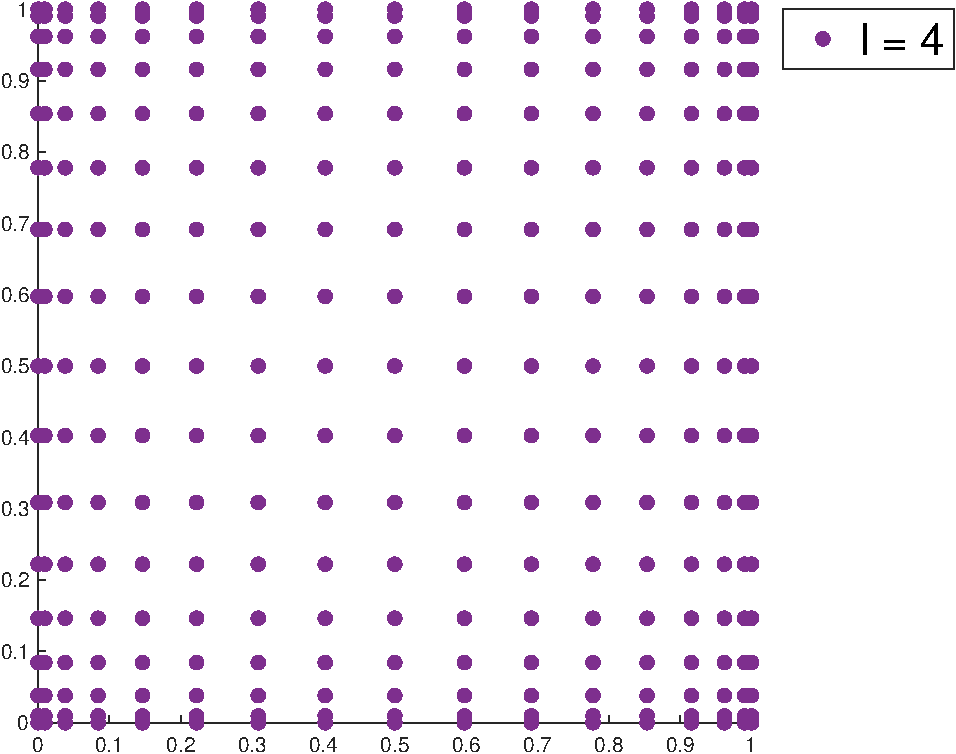
\includegraphics[width=0.2\linewidth]{./figures_slides/full_grid_2d}
            &
            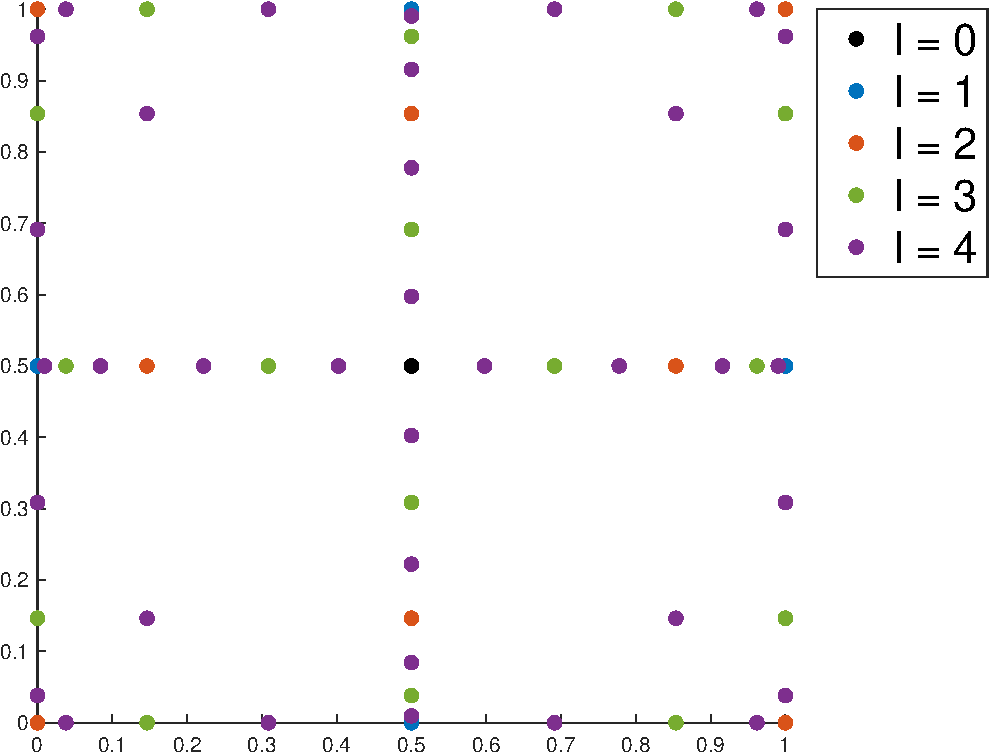
\includegraphics[width=0.2\linewidth]{./figures_slides/sparse_grid_2d}
            &
            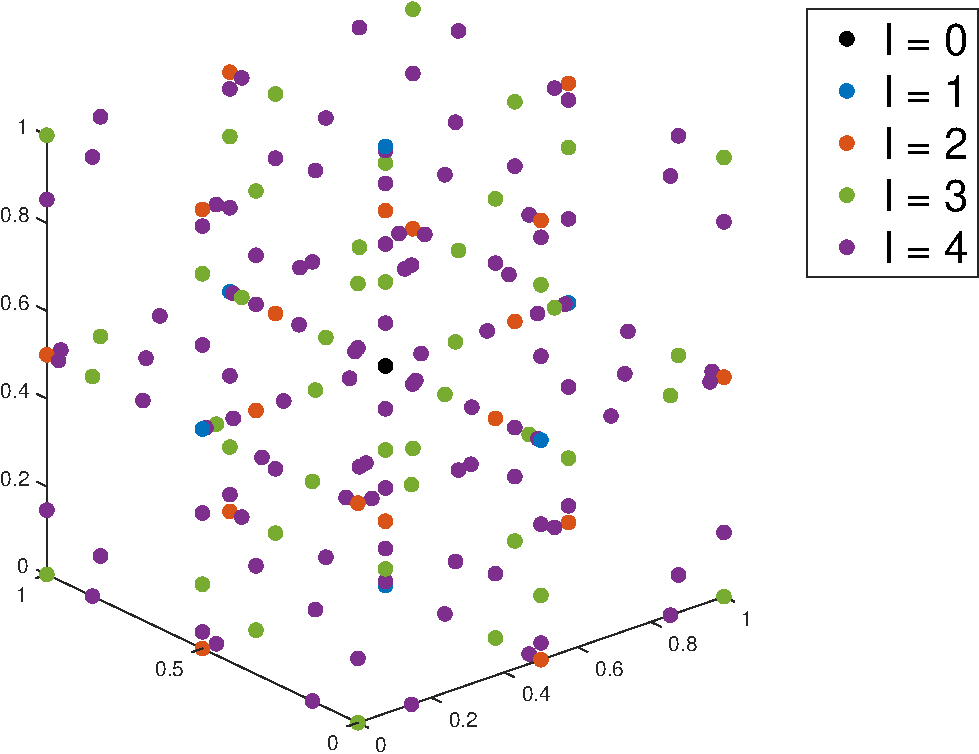
\includegraphics[width=0.2\linewidth]{./figures_slides/sparse_grid_3d}
        \end{tabular}
        \vspace{-3mm}
        \caption*{{\fontsize{8}{8}\selectfont  Left to right: Full tensor grid 2d, level 4. Chebyshev sparse grids for 2d and 3d from level 0 to level 4. \par}}
        \end{figure}

        \vspace{-6mm}
        \fbox{%
        \parbox{1.01\textwidth}{
        \textcolor{myblue3}{\bf Theorem:} {\footnotesize Interpolation error bound in $L_\infty$ norm
        \vspace{-2mm}
        \[\|f-\mathscr{S}(f)\|_\infty = \mathscr{O}\left(N^{-k}\cdot \vert \log N\vert ^{(k+2)(d-1) +1}\right)\vspace{-2mm}\]
        $N$: \# of collocation nodes, $d$: dimension, $k$: measure of smoothness of $\psi$ wrt $\boldsymbol{\omega}$.}}}

    
        
        % {\fontsize{8}{8}\selectfont  \textcolor{mygray2}{V. Barthelmann, E. Novak, and K. Ritter. High dimensional polynomial interpolation on sparse grids. Advances in Computational Mathematics, 12:273–288, 2000.}
        % \par}

        \vspace{2mm}
        \item[$\circ$] {\bf Software:} {\footnotesize \textsc{Matlab} {\tt SPINTERP}  package -- A.Klimke.}
        
        \vspace{1mm}
        {\fontsize{8}{8}\selectfont \textcolor{mygray2}{SPINTERP, piecewise multilinear hierarchical sparse grid interpolation, http://people.math.sc.edu/burkardt/msrc/spinterp/spinterp.html, 2007.}
        \par}
        % \item [$\circ$] \textcolor{myblue3}{\bf Reference}: 
        % {\footnotesize V. Barthelmann and his collaborators.\par}
        
    
    \end{itemize}

\end{itemize}
\end{frame}


% %------------------------------------------------------------
% \begin{frame}[t]
%     \frametitle{Multi-fidelity Monte Carlo}

%     \begin{itemize}[leftmargin=5pt] 
%      \vspace{3mm}
%         \item[$\triangleright$] How It Works:
%         \begin{itemize}[leftmargin=15pt]
%             \item[$\circ$] Multiple Fidelity Levels: It leverages models of different fidelities—e.g., simplified physics-based models, surrogate models, or coarse-grid simulations.
            
%             \item[$\circ$] Control Variate Approach: The low-fidelity models act as control variates to correct and improve estimates from the expensive high-fidelity model.

%             \item[$\circ$] Optimal Sampling Strategy: MFMC determines the optimal number of simulations to run at each fidelity level to achieve the best trade-off between accuracy and cost.
%         \end{itemize}

%     \end{itemize}


% \end{frame}


%------------------------------------------------------------
\begin{frame}[t]
    \frametitle{Multi-fidelity Monte Carlo}
    {\footnotesize Let $\Delta_k = \rho_{1,k}^2 - \rho_{1,k+1}^2$ for $k = 1, \dots, K$, with $\rho_{1,K+1} = 0$.}
    \begin{itemize}[leftmargin=5pt] 
     \vspace{3mm}
        \item[$\triangleright$] \textcolor{myblue3}{\bf The original optimization problem:}
        {\footnotesize
                %
        \begin{equation*}\label{eq:Optimization_pb_sample_size}
            \begin{array}{ll}
            \min \limits_{\begin{array}{c}
        \scriptstyle \alpha_2,\ldots,\alpha_K\in \mathbb{R}
        \end{array}} &\mathbb{V}\left[A^{\text{MF}}\right]=\sigma_1^2\sum_{k=1}^K\frac{\Delta_{k}}{N_k},\\
               \;\,\text{subject to} &\displaystyle\sum\limits_{k=1}^K C_kN_k=p,\\[2pt]
               &\displaystyle -N_1\le 0,\quad \displaystyle N_{k-1}-N_k\le 0, \;\; k=2\ldots,K,\\
               &N_1,\ldots, N_K\in \mathbb{R}. 
            \end{array}
        \end{equation*}
        %
        }

        \item[$\triangleright$] \textcolor{myblue3}{\bf  Ours:}
        {\footnotesize
                %
        \begin{equation*}\label{eq:Optimization_pb_sample_size}
            \begin{array}{ll}
            \min \limits_{\begin{array}{c}
        \scriptstyle \alpha_2,\ldots,\alpha_K\in \mathbb{R}
        \end{array}} &\sum\limits_{k=1}^K C_kN_k,\\
               \;\,\text{subject to} &\displaystyle\mathbb{V}\left[A^{\text{MF}}\right]=\epsilon_{\text{tar}}^2,\\[2pt]
               &\displaystyle -N_1\le 0,\quad \displaystyle N_{k-1}-N_k\le 0, \;\; k=2\ldots,K,\\
               &N_1,\ldots, N_K\in \mathbb{R}. 
            \end{array}
        \end{equation*}
        %
        }
        
    \end{itemize}
\end{frame}


%------------------------------------------------------------
\begin{frame}[t]
    \frametitle{MFMC Optimal Sample Allocation}
    % \begin{itemize}[leftmargin=5pt] 
    %  \vspace{3mm}
    %     \item[$\triangleright$] The original optimization problem
        {\fontsize{8}{8}\selectfont 
        %
        \begin{theorem}[Original problem -- Simplified sample size]
        \label{thm:Sample_size_est}
        Consider an ensemble of $K$ models $\{u_{h,k}\}_{k=1}^K$ each characterized by the standard deviation $\sigma_k$ of its output, the correlation coefficient $\rho_{1,k}$ with the highest-fidelity model $u_{h,1}$, and the computational cost per sample evaluation $C_k$. Define $\Delta_k = \rho_{1,k}^2 - \rho_{1,k+1}^2$ for $k = 1, \dots, K$, with $\rho_{1,K+1} = 0$. Assume the following conditions hold
        \vspace{-5mm}
        
        %
        \begin{alignat*}{3}
        &(i)\;\; \textit{Correlation monotonicity}: \quad && |\rho_{1,1}| > \cdots > |\rho_{1,K}|, \\ 
        &(ii)\;\; \textit{Cost-correlation ratio}: \quad && \frac{\Delta_{k}}{C_k} > \frac{\Delta_{k-1}}{C_{k-1}}, \quad k=2,\ldots,K. 
        \end{alignat*}
        %
        
        \vspace{-3mm}
        Under these assumptions, the solution to the original optimization problem  yields optimal weights $\alpha_k^*=\frac{\rho_{1,k}\sigma_1}{\sigma_k}$.
        % %
        % \begin{align}
        %     % \label{eq:MFMC_coefficients}
        %     % &\alpha_k^*=\frac{\rho_{1,k}\sigma_1}{\sigma_k},\\
        %     \label{eq:MFMC_SampleSize}
        %     &\alpha_k^*=\frac{\rho_{1,k}\sigma_1}{\sigma_k},
        % \end{align}
        % %
        define an intermediate vector $\boldsymbol{r}^* = [r_1,\ldots,r_k]^T$, then $\boldsymbol{r}^*$ and the sample sizes $N_k^*$
        \vspace{-3mm}
        %
        \[
        r_k^* = \sqrt{\frac{C_1\Delta_k}{C_k\Delta_1}},\quad N_1^* = \frac{p}{\sum_{k=1}^K C_k r^*_k}, \quad N_k^*=N_1^*r_k^*,\quad \Rightarrow \quad \JLcolor{N_k^* = \sqrt{\frac{\Delta_k}{C_k}}\frac{p}{\sum_{j=1}^K \sqrt{C_j\Delta_j}}}.
        \] 
        \vspace{-3mm}
        %
        The resulting MFMC estimator achieves a variance of
        %
        \begin{equation*}
        \label{eq:MFMC_variance_optimal}
        \mathbb{V}\left[A^{\text{MF}}\right] =
        % \frac{\sigma_1^2}{N_1^*} - \sum_{k=2}^K \left(\frac{1}{N_{k-1}^*} - \frac{1}{N_k^*}\right)\rho_{1,k}^2\sigma_1^2=
        \frac{\sigma_1^2}{p}\left(\sum_{k=1}^K\sqrt{C_k\Delta_{k}}\right)^2.
        \end{equation*}
        %
        \end{theorem}
        }

\end{frame}



% %------------------------------------------------------------
% \begin{frame}[t]
%     \frametitle{MFMC Optimal Sample Allocation}
%     % \begin{itemize}[leftmargin=5pt] 
%     %  \vspace{3mm}
%     %     \item[$\triangleright$] The original optimization problem
%         {\fontsize{8}{8}\selectfont 
%         %
%         \begin{theorem}[Original problem -- Simplified sample size]
%         \label{thm:Sample_size_est}
%         Consider an ensemble of $K$ models $\{u_{h,k}\}_{k=1}^K$ each characterized by the standard deviation $\sigma_k$ of its output, the correlation coefficient $\rho_{1,k}$ with the highest-fidelity model $u_{h,1}$, and the computational cost per sample evaluation $C_k$. Define $\Delta_k = \rho_{1,k}^2 - \rho_{1,k+1}^2$ for $k = 1, \dots, K$, with $\rho_{1,K+1} = 0$. Assume the following conditions hold
%         \vspace{-5mm}
        
%         %
%         \begin{alignat*}{3}
%         &(i)\;\; \textit{Correlation monotonicity}: \quad && |\rho_{1,1}| > \cdots > |\rho_{1,K}|, \\ 
%         &(ii)\;\; \textit{Cost-correlation ratio}: \quad && \frac{\Delta_{k}}{C_k} > \frac{\Delta_{k-1}}{C_{k-1}}, \quad k=2,\ldots,K. 
%         \end{alignat*}
%         %
        
%         \vspace{-3mm}
%         Under these assumptions, the solution to the original optimization problem  yields optimal weights $\alpha_k^*=\frac{\rho_{1,k}\sigma_1}{\sigma_k}$.
%         % %
%         % \begin{align}
%         %     % \label{eq:MFMC_coefficients}
%         %     % &\alpha_k^*=\frac{\rho_{1,k}\sigma_1}{\sigma_k},\\
%         %     \label{eq:MFMC_SampleSize}
%         %     &\alpha_k^*=\frac{\rho_{1,k}\sigma_1}{\sigma_k},
%         % \end{align}
%         % %
%         The sample sizes $N_k^*$ and variance are
%         \vspace{-3mm}
%         %
%         \[
%         \JLcolor{N_k^* = \sqrt{\frac{\Delta_k}{C_k}}\frac{p}{\sum_{j=1}^K \sqrt{C_j\Delta_j}}},\quad \mathbb{V}\left[A^{\text{MF}}\right] =
%         % \frac{\sigma_1^2}{N_1^*} - \sum_{k=2}^K \left(\frac{1}{N_{k-1}^*} - \frac{1}{N_k^*}\right)\rho_{1,k}^2\sigma_1^2=
%         \frac{\sigma_1^2}{p}\left(\sum_{k=1}^K\sqrt{C_k\Delta_{k}}\right)^2.
%         \] 
%         % \vspace{-3mm}
%         % %
%         % The resulting MFMC estimator achieves a variance of
%         % %
%         % \begin{equation*}
%         % \label{eq:MFMC_variance_optimal}
%         % \mathbb{V}\left[A^{\text{MF}}\right] =
%         % % \frac{\sigma_1^2}{N_1^*} - \sum_{k=2}^K \left(\frac{1}{N_{k-1}^*} - \frac{1}{N_k^*}\right)\rho_{1,k}^2\sigma_1^2=
%         % \frac{\sigma_1^2}{p}\left(\sum_{k=1}^K\sqrt{C_k\Delta_{k}}\right)^2.
%         % \end{equation*}
%         % %
%         \end{theorem}
%         }

% \end{frame}




%------------------------------------------------------------
\begin{frame}[t]
    \frametitle{MFMC Optimal Sample Allocation}
    % \begin{itemize}[leftmargin=5pt] 
    %  \vspace{3mm}
    %     \item[$\triangleright$] The original optimization problem
        {\fontsize{8}{8}\selectfont 
        %
        \begin{theorem}[Our problem]
        \label{thm:Sample_size_est}
        Consider an ensemble of $K$ models $\{u_{h,k}\}_{k=1}^K$ each characterized by the standard deviation $\sigma_k$ of its output, the correlation coefficient $\rho_{1,k}$ with the highest-fidelity model $u_{h,1}$, and the computational cost per sample evaluation $C_k$. Define $\Delta_k = \rho_{1,k}^2 - \rho_{1,k+1}^2$ for $k = 1, \dots, K$, with $\rho_{1,K+1} = 0$. Assume the following conditions hold
        \vspace{-5mm}
        
        %
        \begin{alignat*}{3}
        &(i)\;\; \textit{Correlation monotonicity}: \quad && |\rho_{1,1}| > \cdots > |\rho_{1,K}|, \\ 
        &(ii)\;\; \textit{Cost-correlation ratio}: \quad && \frac{\Delta_{k}}{C_k} > \frac{\Delta_{k-1}}{C_{k-1}}, \quad k=2,\ldots,K. 
        \end{alignat*}
        %
        
        \vspace{-3mm}
        Under these assumptions, the solution to the original optimization problem  yields optimal weights $\alpha_k^*=\frac{\rho_{1,k}\sigma_1}{\sigma_k}$.
        % %
        % \begin{align}
        %     % \label{eq:MFMC_coefficients}
        %     % &\alpha_k^*=\frac{\rho_{1,k}\sigma_1}{\sigma_k},\\
        %     \label{eq:MFMC_SampleSize}
        %     &\alpha_k^*=\frac{\rho_{1,k}\sigma_1}{\sigma_k},
        % \end{align}
        % %
        The sample sizes $N_k^*$ and total computational cost are
        \vspace{-3mm}
        %
        \[
        N_k^*=\frac{\sigma_1^2}{\epsilon_\text{tar}^2}\sqrt{\frac{\Delta_{k}}{C_k}}\sum_{j=1}^K\sqrt{C_j\Delta_{j}}, \qquad \mathcal{W}^\text{MF} = \frac{\sigma_1^2}{\epsilon_{\text{tar}}^2}\left(\sum_{k=1}^K\sqrt{C_k\Delta_{k}}\right)^2.
        \] 
        % \vspace{-3mm}
        % %
        % The total computational cost is
        % %
        % \begin{equation*}
        % \label{eq:MFMC_variance_optimal}
        % \mathcal{W}^\text{MF} = \frac{\sigma_1^2}{\epsilon_{\text{tar}}^2}\left(\sum_{k=1}^K\sqrt{C_k\Delta_{k}}\right)^2.
        % \end{equation*}
        % %
        \end{theorem}
        }
        {\footnotesize
        \begin{itemize}[leftmargin=5pt] 
            \item[$\circ$] Convex problem $\rightarrow$ unique solution.
            \item[$\circ$] Sample sizes $N_k^*$ increase monotonically with fidelity level.
            \item[$\circ$] Global optimality established via KKT and block-structure analysis.
        \end{itemize}
        }
\end{frame}


\begin{frame}{Rounding \& Example}
\begin{itemize}[leftmargin=5pt] 
\item[$\triangleright$] Closed-form $N_k^*$ are real $\rightarrow$ need integer rounding.

\item[$\triangleright$] Parameters
\renewcommand{\arraystretch}{2}
\begin{table}[ht]
\centering
\scalebox{0.6}{
\begin{tabular}{|c|c|c|c|c|c|c|}
\hline
Model index &1 &2 &3 &4 &5 \\
\hline
Correlation coeff $\rho_{1,k}$ &1     &9.9977e-01   &9.9925e-01  &9.9728e-01   &9.8390e-01\\
\hline
Standard deviation $\sigma_k$ &1.0840e-02    &1.0838e-02   &1.1001e-02  &1.1549e-02   &9.5720e-03\\
\hline
Cost &73&7.0318e-03 &1.4018e-03 &5.0613e-04 &2.6803e-04\\
\hline
\end{tabular}
}
% \caption{Parameters from plasma problem.}
\label{Tab:Parameters}
\end{table}

 \item[$\triangleright$] Sample size
%
\begin{table}[ht]
\centering
\scalebox{0.52}{
\begin{tabular}{|c|c|c|c|c|c|c|c|c|c|}
\hline
&Sample size &Total cost $p$ &$\mathbb{V}\left[A^{\text{MF}}\right]$\\
\hline
Real valued &[8.8130e-01,   1.3499e+02,   5.8811e+02,   2.5409e+03, 2.1100e+04]&\cellcolor{blue!40} 73.05&\cellcolor{yellow!} 6.9633e-08\\
\hline
Real valued, floor &[0,   134,   588,   2540,  21100]&\cellcolor{blue!20} 8.7075&$\infty$\\
\hline
Modified MFMC &[1,   1,   3,    13,   114]&\cellcolor{blue!20}73.0484&1.5677e-06\\
% \hline
\hline
Integer program &[1, 2, 3, 11, 97]&\cellcolor{blue!20}73.0498&1.7250e-06\\
\hline
\hline
Real valued, ceil &[1,   135,   589,   2541,  21101]&81.7167&\cellcolor{yellow!30}6.2353e-08\\
% CPU time for integer program [s] & 0.27\\
\hline
\end{tabular}
}
% \caption{Sample size for real-valued optimization and integer optimization for $p=73.05$.}
\label{Tab:Sample_Size_1}
\end{table}
%
\item[$\triangleright$] Ours: Simple rounding technique preserves variance constraint, adds negligible overhead to computational cost.
\end{itemize}
\end{frame}


%------------------------------------------------------------
\begin{frame}[t]
    \frametitle{Modified MFMC}

    
    \begin{algorithm}[H]
    {\fontsize{8}{8}\selectfont 
    \begin{algorithmic}[1]

    \REQUIRE Parameters $\rho_{1,k}$ and $C_k$ for each $\widehat u_{h, k}$, total cost $p$. Ensure the $K$ models $\widehat u_{h, k}$ after the model selection satisfies $p\ge \sum_i C_i$.

    \ENSURE Sample sizes $N_k$ for $K$ models.

    \vspace{2mm}
    
    \STATE Set the weights $\alpha_k = \frac{\rho_{1,k}\sigma_1}{\sigma_k}, \quad 1\le k\le K.$

    \WHILE{there is $1\le j\le K-1$ such that $N_j<1$}
    
    \STATE  Set $j$ equal to the first such index.
    \STATE  $N_j\gets 1$. 
    \STATE  Set the $k$-st component of $N_k$,
            \[
            N_{k} = \sqrt{\frac{\Delta_{k}}{C_{k}}}\frac{p-\sum_{i=1}^j C_i}{\sum_{i=j+1}^{K} \sqrt{C_i\Delta_i}}, \qquad j+1\le k\le K.
            \]
    \ENDWHILE
    
    \end{algorithmic}
    \caption{Modified MFMC}
    % \label{alg:seq}
    }
    \end{algorithm}
    
\end{frame}

%------------------------------------------------------------
\begin{frame}[t]
    \frametitle{Summary for MFMC formulations}
\renewcommand{\arraystretch}{2.3}
\begin{table}[ht]
\centering
\scalebox{0.6}{
\begin{tabular}{|c|c|c|c|}
\hline
& \multirow{2}{*}{Original} 
& \multirow{2}{*}{Modified MFMC } 
& \multirow{2}{*}{Ours} \\
& &(due to decimal sample size btw $0\sim 1$) & \\
\hline
$\displaystyle\mathbb{V}\left[A^{\text{MF}}\right]$ 
& $\displaystyle\frac{\sigma_1^2}{p}\left(\sum_{k=1}^K\sqrt{C_k\Delta_{k}}\right)^2$ 
& $\sigma_1^2\sum_{k=1}^K\frac{\Delta_{k}}{N_k}$ 
& $\epsilon_{\text{tar}}^2$ \\
\hline
$\displaystyle \mathcal{W}^\text{MF}$ 
& $p$ 
& $\le p$ 
& $\displaystyle\frac{\sigma_1^2}{\epsilon_{\text{tar}}^2}\left(\sum_{k=1}^K\sqrt{C_k\Delta_{k}}\right)^2$ \\
\hline
\multirow{3}{*}{$N_k$} 
& \multirow{3}{*}{$\displaystyle\sqrt{\frac{\Delta_k}{C_k}}\frac{p}{\sum_{j=1}^K \sqrt{C_j\Delta_j}}$} 
& \multirow{3}{*}{\parbox{0.6\linewidth}{%
While there is $1\le j\le K-1$ such that $N_j<1$, set $N_j\gets 1$ and update
\[
   \sqrt{\tfrac{\Delta_{k}}{C_{k}}}\,
   \frac{p-\sum_{i=1}^j C_i}{\sum_{i=j+1}^{K} \sqrt{C_i\Delta_i}},\quad j+1 \le k \le K.
\]
% for $j+1 \le k \le K$.
}
} 
& \multirow{3}{*}{$\displaystyle\frac{\sigma_1^2}{\epsilon_\text{tar}^2}\sqrt{\frac{\Delta_{k}}{C_k}}
   \sum_{j=1}^K\sqrt{C_j\Delta_{j}}$} \\
& & & \\
& & & \\
\hline
Rounding 
& Floor 
& Floor 
& Ceil  \\
\hline
\end{tabular}
}
\label{Tab:Sample_Size2}
\end{table}
\end{frame}


%------------------------------------------------------------
\begin{frame}[c]
\setbeamercolor{itemize item}{fg=mygray1}
\large 	
\textcolor{mygray1}{
    \begin{itemize}[leftmargin=5pt] 
        \item[$\triangleright$]  Physical Model: Grad-Shafranov Equation
        \vspace{0.2cm}	
        \item[$\triangleright$] Uncertainty Quantification
        \vspace{0.2cm}
        \item[$\triangleright$]  Objectives \& Approaches
        \vspace{0.2cm}
        \item[$\triangleright$] Multi-fidelity Monte Carlo
            % \vspace{0.3cm}
            % {\footnotesize
            % \begin{itemize}[leftmargin=15pt]   
            %     \item[$\circ$] Surrogate via Sparse Grid Stochastic Collocation
            %     % \vspace{0.3cm}
            %     \item[$\circ$] Experimental Results \& Conclusions
            % \end{itemize}
            % }
        \vspace{0.2cm}
        \item[\textcolor{black}{$\triangleright$}] \textcolor{black}{\fontsize{25}{60}\selectfont Parameter Estimation}
            % \vspace{0.3cm}
            % {\footnotesize
            % \begin{itemize}[leftmargin=15pt]   
            %     \item[$\circ$] Monte Carlo \& Uniform Multilevel Monte Carlo
            %     \item[$\circ$] Adaptive Multilevel Monte Carlo
            %     \item[$\circ$] Experimental Results \& Conclusions
            % \end{itemize}
            % }
        \vspace{0.2cm}
        \item[$\triangleright$] Numerical Results
            % {\footnotesize
            % \begin{itemize}[leftmargin=15pt]   
            %     \item[$\circ$] Three Types of Surrogates
            %     \item[$\circ$] Surrogate-based Samplings
            %     \item[$\circ$] Experimental Results \& Conclusions
            % \end{itemize}
            % }
        % \vspace{0.2cm}
        % \item[$\triangleright$] Approach 4: Multi-fidelity Monte Carlo
    \end{itemize}
}
\end{frame}
%------------------------------------------------------------


%------------------------------------------------------------
\begin{frame}[t]
\frametitle{Parameter Estimation}
{\footnotesize
\begin{itemize}[leftmargin=5pt] 
\item[$\triangleright$] Parameters to estimate: $C_k$, $\sigma_k$, $\rho_{1,k}$.
\item[$\triangleright$] Sample standard deviation and cost: unbiased, converge quickly.
\item[$\triangleright$] \textcolor{myblue3}{\bf Sample correlation coefficient}: biased, skewed distribution mean $|\rho_{1,k}|\rightarrow 1$. Requires careful pilot sampling to avoid efficiency loss.
%
\[
\widehat{\rho}_{1,k} = \frac{\sum_{i=1}^Q\left\langle u_{1}^{(i)} - A_{1,Q}^{\text{MC}},\; u_{k}^{(i)} - A_{k,Q}^{\text{MC}} \right\rangle_U}{\sqrt{\sum_{i=1}^Q \left\|u_{1}^{(i)} - A_{1,Q}^{\text{MC}}\right\|_U^2} \sqrt{\sum_{i=1}^Q \left\|u_{k}^{(i)} - A_{k,Q}^{\text{MC}}\right\|_U^2}},
\]
%
$Q$: number of pilot samples,

$u_k^{(i)}$: $i$-th realization of the $k$-th model,

\item[$\triangleright$] \textcolor{myblue3}{\bf Dynamic Pilot Sampling Strategy}

\begin{itemize}[leftmargin=15pt] 
            \item[$\circ$] Sequentially increase pilot sample size until the relative cost efficiency update falls below certain threshold using sensitivity of cost efficiency.
            % \item[$\circ$] Use Fisher $z$-transform/Bootstrap to build confidence intervals for double check.
            \item[$\circ$] Avoids unnecessary large pilot runs while ensuring reliability. Achieves accuracy comparable to fixed-$Q$ but at lower cost.
        \end{itemize}
\end{itemize}
}
\end{frame}


%------------------------------------------------------------
\begin{frame}[c]
\setbeamercolor{itemize item}{fg=mygray1}
\large 	
\textcolor{mygray1}{
    \begin{itemize}[leftmargin=5pt] 
        \item[$\triangleright$]  Physical Model: Grad-Shafranov Equation
        \vspace{0.2cm}	
        \item[$\triangleright$] Uncertainty Quantification
        \vspace{0.2cm}
        \item[$\triangleright$] Objectives \& Approaches
        \vspace{0.2cm}
        \item[$\triangleright$]  Multi-fidelity Monte Carlo
            % \vspace{0.3cm}
            % {\footnotesize
            % \begin{itemize}[leftmargin=15pt]   
            %     \item[$\circ$] Surrogate via Sparse Grid Stochastic Collocation
            %     % \vspace{0.3cm}
            %     \item[$\circ$] Experimental Results \& Conclusions
            % \end{itemize}
            % }
        \vspace{0.2cm}
        \item[$\triangleright$] Parameter Estimation
            % \vspace{0.3cm}
            % {\footnotesize
            % \begin{itemize}[leftmargin=15pt]   
            %     \item[$\circ$] Monte Carlo \& Uniform Multilevel Monte Carlo
            %     \item[$\circ$] Adaptive Multilevel Monte Carlo
            %     \item[$\circ$] Experimental Results \& Conclusions
            % \end{itemize}
            % }
        % \vspace{0.2cm}
        % \item[$\triangleright$]  Numerical Results
            % {\footnotesize
            % \begin{itemize}[leftmargin=15pt]   
            %     \item[$\circ$] Three Types of Surrogates
            %     \item[$\circ$] Surrogate-based Samplings
            %     \item[$\circ$] Experimental Results \& Conclusions
            % \end{itemize}
            % }
        \vspace{0.2cm}
        \item[\textcolor{black}{$\triangleright$}] \textcolor{black}{\fontsize{25}{60}\selectfont Numerical Results}
    \end{itemize}
}
\end{frame}
%------------------------------------------------------------
% %------------------------------------------------------------
% \begin{frame}[t]
%     \frametitle{Dynamic Pilot Sampling Strategy}
%     %
% \begin{algorithm}[H]
%     {\fontsize{8}{8}\selectfont 
%     \begin{algorithmic}[1]

    
    
%     \vspace{1mm}
%     \hrule
%     \vspace{1mm}
     
%     \STATE Initialization:\\

%     \STATE\hspace{3mm}\textbullet~ $dQ \gets Q_0$, $p \gets 0$, $\text{converged} \gets \texttt{False}$, $\text{stable}\_\text{count} \gets 0$, $\mathcal{I}^{prev}\gets \emptyset$. %\tcp*{}
    
%     \STATE\hspace{3mm}\textbullet~  Welford's initialization: $m_k^{(0)} \gets 0$, $v_k^{(0)} \gets 0$ for $k=1,\dots,K_c$,  $r_k^{(0)} \gets 0$, for $k=2,\dots,K_c$. %\tcp*{Welford's algorithm}



% \WHILE{$\neg \text{converged}$ \& $\text{stable}\_\text{count}< \tau$}
    
%     \FOR{$k=2,\ldots, K_c$}
    
%         \FOR{$i = 1,\cdots, dQ $}
    
%         \STATE $Q \gets  p+i$.

%         \STATE Draw $dQ$ new samples $\{\boldsymbol{\omega}^{(i)}\}_{i=1}^{dQ}$, compute sample realization $u_{1}^{(Q)}$ and $u_{k}^{(Q)}$.\\

%         \STATE Update mean $m_1^{(Q)}$, $m_k^{(Q)}$, proxies $v_1^{(Q)}$, $v_k^{(Q)}$ and $r_{k}^{(Q)}$ via Welford's algorithm.
        
%         \ENDFOR
    
%     \STATE Compute correlations: $\widehat\rho_{1,k}^{(Q)}\gets r_k^{(Q)}/{\sqrt{v_1^{(Q)}v_k^{(Q)}}}$ for $k=2,\ldots, K_c$. 

    
    
%     % \eIf{bivariate normality holds}{
        
%     %         $\widehat{z}_k \gets \tanh^{-1}\left(\widehat{\rho}_{1,k}^{(Q)}\right)$, $\sigma_{\widehat{z}_k} \gets 1/\sqrt{Q - 3}$. \\
%     %         Compute confidence interval $\text{CI}_{\rho_{1,k}}^{\text{fisher}}$ and its width $t_k$ via Fisher z-transform in \eqref{eq:Confidence_Interval_fisher}.
        
%     % }{
        
%     %         Generate $B$ bootstrap replicates of $\widehat{\rho}_{1,k}^{(Q)}$.  \\
%     %         Compute  confidence interval $\text{CI}_{\rho_{1,k}}^{\text{boot}}$ and its width $t_k$ via bootstrap in \eqref{eq:Confidence_Interval_bootstrap}.
        
%     % }
%     }

%     \STATE $\widehat{\boldsymbol{\rho}}^{(Q)} \gets (1,\widehat{\rho}_{1,2}^{(Q)}, \dots, \widehat{\rho}_{1,K_c}^{(Q)})$.

%     % $\delta \gets \frac{2\vartheta}{E\sqrt{K-1}}$
%     % [$\text{index},\xi^{(p)}$] = Multi-fidelity Model Selection ($\boldsymbol{\rho}^{(p)},\boldsymbol{C}$).

%     % $Q \geq \max\{30, Q_{\max \{\text{idx}^{current}\}} \}$ \text{as in } \eqref{eq:Pilot_sample_size_estimate} and
%     \STATE $\left[\mathcal{I}^{cur},\widehat{\xi}^{(Q)}\right]$ $\gets$ \textsc{ModelSelectionBacktrack} $\left(\widehat{\boldsymbol{\rho}}^{(Q)},\boldsymbol{C}\right)$.\\

%     \eIf{$\frac{\widehat \xi^{(Q)}- \widehat \xi^{(p)}}{\widehat \xi^{(Q)}}\leq \vartheta$, $\mathcal{I}^{prev}=\mathcal{I}^{cur}$ }{ %$\max_k t_k \leq \delta$
%             $\text{converged} \gets \texttt{True}$.

%             $\text{stable}\_\text{count} \gets  \text{stable}\_\text{count}+1$.
%     }
%     {
%             $\text{stable}\_\text{count} \gets  0$.
    
%         $p \gets  p+dQ$. %\tcc*{Increase sample size.}
        
%         $\widehat{\xi}^{(p)} \gets  \widehat{\xi}^{(Q)}$.
%     }
    

%     $\mathcal{I}^{prev} \gets \mathcal{I}^{cur}$.

%     \ENDWHILE
    
% $\widehat{\sigma}_1 \gets \sqrt{v_1^{(Q)}}$, $\widehat{\sigma}_k \gets \sqrt{v_k^{(Q)}}$, $\widehat{\alpha}_k \gets \widehat{\rho}_{1,k}^{(Q)} \widehat{\sigma}_1^{(Q)} / \widehat{\sigma}_k^{(Q)}$, for $k \in \mathcal{I}^{cur}$.

% Return $\widehat{\boldsymbol{\sigma}} \gets [\widehat{\sigma}_1,\ldots,\widehat{\sigma}_{K}]$, $\widehat{\boldsymbol{\alpha}} \gets [1,\widehat{\sigma}_2\ldots,\widehat{\sigma}_{K}]$, $\widehat{\boldsymbol{\rho}} \gets \widehat{\boldsymbol{\rho}}^{(Q)}$, $\widehat{\xi} \gets \widehat{\xi}^{(Q)}$, $\mathcal{I} \gets \mathcal{I}^{cur}$.

%     \end{algorithmic}
%     \caption{Dynamic Parameter Estimation}
%     }
%     \end{algorithm}

% \end{frame}





% \begin{frame}
% \frametitle{Dynamic Parameter Estimation - Part 1}


% \begin{algorithm}[H]
%     \caption{Dynamic Parameter Estimation}
%     {\fontsize{8}{8}\selectfont 
%     \begin{algorithmic}[1]
%         \REQUIRE Relative error $\vartheta$ in $\xi$, number of models $K_c$, initial sample size $Q_0$, cost vector $\boldsymbol{C} = (C_1, \dots, C_{K_c})$, stability threshold $\tau=3$.
        
%         \ENSURE Final sample size $Q$, estimated parameters $\widehat{\boldsymbol{\sigma}},\widehat{\boldsymbol{\alpha}}, \widehat{\boldsymbol{\rho}}$, efficiency $\widehat{\xi}$, model index set $\mathcal{I}$.

%         \STATE Initialization:\\
%     \STATE\hspace{3mm}\textbullet~ $dQ \gets Q_0$, $p \gets 0$, $\text{converged} \gets \texttt{False}$, $\text{stable}\_\text{count} \gets 0$, $\mathcal{I}^{prev}\gets \emptyset$. %\tcp*{}
    
%     \STATE\hspace{3mm}\textbullet~  Welford's initialization: $m_k^{(0)} \gets 0$, $v_k^{(0)} \gets 0$ for $k=1,\dots,K_c$,  $r_k^{(0)} \gets 0$, for $k=2,\dots,K_c$. 
    
%         \For{$i=1$ to $N$}
%             \State Do something
%             \State Perform calculations
%             \State Store intermediate results
%         \EndFor
%         \State Check condition
%     \end{algorithmic}
%     }
% \end{algorithm}

% \end{frame}

% \begin{frame}
% \frametitle{My Long Algorithm - Part 2}
% \begin{algorithm}[H]
%     \ContinuedFloat % Continues the numbering from the previous algorithm environment
%     \caption{Example Long Algorithm (cont.)}
%     \begin{algorithmic}[1]
%         \State Continue processing
%         \If{condition is met}
%             \State Execute specific steps
%         \Else
%             \State Handle alternative case
%         \EndIf
%         \State Finalize results
%         \State Return output
%     \end{algorithmic}
% \end{algorithm}
% \end{frame}







% \begin{frame}[t]{stellar}
% \frametitle{Necessary conditions -- $t_f$ free}
% {\footnotesize
% \begin{itemize}[leftmargin=5pt] 
%     \item[] 
%     \begin{align*}
%     \text{Lagrangian} \quad &J = \varphi + \nu_b^Tb + \nu_p^T p + \nu_s^T s+\\ 
%     &\int_{t_0}^{t_f}  L + \lambda^t \left[f - \dot{x}\right] 
%     \;dt\\
%         \text{Hamiltonian} \quad &H(t, x, u, \lambda) = L(t, x, u) + \lambda(t)^T f(t, x, u),\\
%          \text{Control} \quad &u^* = \operatorname*{argmin}_{u\in \mathcal{U}}\, H(t, x^*, u,\lambda^*),\quad \forall t\in[t_0, t_f],\\
%         \text{State} \quad &\dot{x} = \frac{\partial H}{\partial \lambda},\\
%         \text{Adjoint equation} \quad &\dot{\lambda} = -\frac{\partial H}{\partial x},\\
%         \text{T ransversality cond} \quad &\lambda (t_f) = 
%     \end{align*}
% \end{itemize}
% }	
% \end{frame}


%}
%=================================================
% Imagine two positive nuclei in my hand, two forces acting on them: nuclear force (attract them) and coulub force(push them aways), when at big distance, nuclei repel each other, when find ways to conquer the coulomb force barrier, two neulei get closed to each other and merge into one heavier neulcei. mass defect release energy. example: sun. 

%Tokamak: russian word--toroidal chamber with magnetic coils. see below two figures. Inject fuel gas into the chamber and heat with microwave, becomes fluid of particles -- called plasma, high temperature, vibrate fast, high speed easy to overcome coulum repulsion and get closed to each other, and collide to produce energy.
%=================================================
% Q: the distance of repel & attract?


% %------------------------------------------------------------
% \begin{frame}[t]
% \frametitle{Plasma Confinement}
% %		\begin{columns}
% %			\begin{column}{0.8\textwidth}

% During fusion, the hot plasma tends to expand, to prevent it from contacting the reactor wall, it must be confined. 

% \vspace{4mm}
% {\fontsize{13}{13}\selectfont \textcolor{myblue3}{\bf Question: How to maintain confinement of hot plasma?} }

% \vspace{2mm}
% \begin{itemize} [leftmargin=5pt] 
% \vspace{-3mm}
% \item[$\triangleright$] Since plasmas are conductive and magnetically tractable -- use a \textcolor{myred}{\bf magnetic field}  generated by currents in  external coils around the fusion reactor.
% \vspace{1.8mm}

% %When heated to fusion temperatures, the electrons in atoms disassociate, resulting in a fluid of nuclei and electrons known as a plasma. Unlike electrically neutral atoms, a plasma is electrically conductive, and can, therefore, be manipulated by electrical or magnetic fields.
% \item[$\triangleright$] Our project focuses on studying the \textcolor{myred}{\bf impact of variations in current} on the physical properties of the confinement field.


% \begin{equation*}
% \hspace{-11mm}
% \text{Variations}
% \left\{ \begin{array}{l}
% \text{Power supply}\\ [3pt]
% \text{Temperature fluctuations}\\ [3pt]
% \text{Material impurities in the conduction wire}
% \end{array}\right.
% \end{equation*}


% \item []
% %\begin{figure}[H]	
% %	\centering
% %	\begin{tabular}{cc}
% %		\begin{subfigure}{0.45\textwidth}
% %			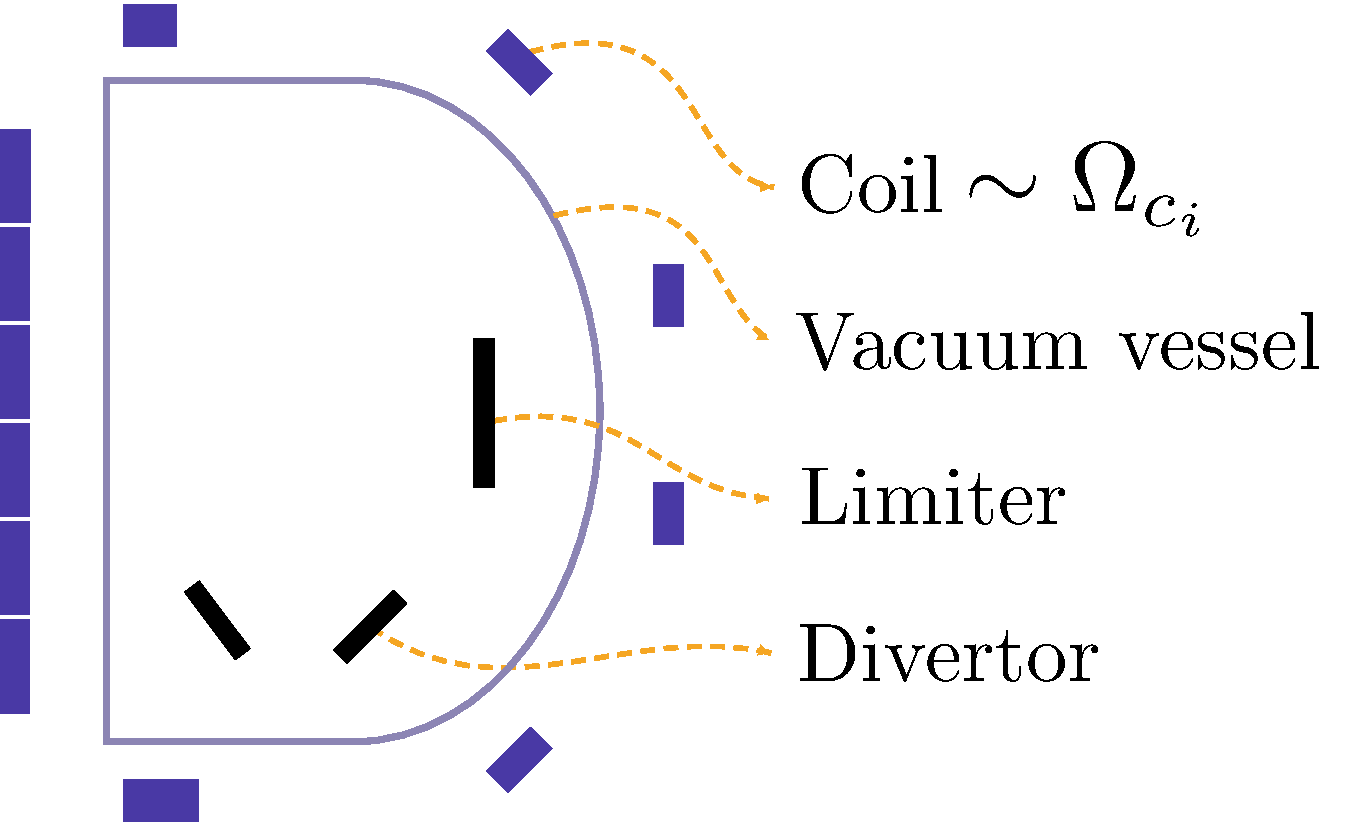
\includegraphics[height=0.55\linewidth]{../../../Project/Plot/BasicConfig}
% %%			\caption*{Divertor configuration}
% %		\end{subfigure}
% %		&
% %		\begin{subfigure}{0.45\textwidth}
% %			\includegraphics[height=0.55\linewidth]{../PictureFolder/PlasmaImage}
% %			\source{https://en.wikipedia.org/wiki/Mega{\_}Ampere{\_}Spherical{\_}Tokamak}
% %%			\caption*{Limiter configuration}
% %		\end{subfigure}
% %	\end{tabular} 
% %\end{figure}
% \end{itemize}
% \end{frame}



%=================================================
% We impose the bottom two conditions. if x is 0, then the equation becomes singular, so the first condition avoid singularity in the equation, and the second equaiton shows the decay of function at infinity, and ensure the uniqueness of the solution.
%=================================================

% %------------------------------------------------------------
% \begin{frame}[t]
%     \frametitle{Uncertainty Quantification (UQ)}
%     \begin{itemize}[leftmargin=5pt]
%         \item[$\triangleright$] \textcolor{myblue3}{\bf Source of uncertainty:} {\footnotesize Investigate the impact of \textcolor{myblue3}{uncertainties in the current intensities} on the confinement properties of a plasma.}
        
%         \item[$\triangleright$] \textcolor{myred}{\bf Baseline current intensities:} 
%         \[
%         \footnotesize
%         \begin{array}{lll}
%         I_1: -1.40\times 10^6\text{A} &I_5: -9.00\times 10^6\text{A} &I_9:  -6.43\times 10^6\text{A} \\
%         I_2: -9.50\times 10^6\text{A} &I_6: 3.56\times 10^6\text{A}  & I_{10}:  -4.82\times 10^6\text{A} \\
%         I_3: -2.04\times 10^7\text{A} &I_7:  5.47\times 10^6\text{A}  &I_{11}:  -7.50\times 10^6\text{A} \\
%         I_4: -2.04\times 10^7\text{A} &I_8: -2.27\times 10^6\text{A} &I_{12}:  1.72\times 10^7\text{A} 
%         \end{array}
%         \]
%         \item[$\triangleright$] \textcolor{myblue3}{\bf Uncertianty Quantification:} {\footnotesize Variations in the baseline current intensities. Each current in the array is considered to be a parameter, so we have 12-dimensional parameter space.}
        
        
%         \item[$\triangleright$] \textcolor{myblue3}{\bf Currents uniformly distributed:} 

%         {\footnotesize
%         \textcolor{mygray3}{$\tau$: perturbation level ($\tau= 1\%$ \& $2\%$). \quad $I_k$: current intensity in the $k$-th coil.}
        

%         \begin{itemize}[leftmargin=15pt]   
%             \item[$\circ$] Joint density function: $\displaystyle
%              \pi \left(\boldsymbol{\omega}\right)=\prod_{k=1}^{d} \pi_k\left(\omega_{k}\right)=\prod_{k=1}^{d} \frac{1}{2\tau |I_k|}$.
%             \item[$\circ$] 12-d parameter space: $\displaystyle W := \prod_{k=1}^{d}\left[I_k-\tau|I_k|,I_k+\tau|I_k|\right]$.
%         \end{itemize}
%         \par}
%     \end{itemize}
% \end{frame}	
%=================================================
% here I list an example of an array of currents, each current in the array is considered to be a parameter, so we have 12 dimensional parameter space, and if we use 1%...., we will use MC method to handle the uncertainty.
%=================================================











% %------------------------------------------------------------
% \begin{frame}[t]
%     \frametitle{Random space: from infinite to finite dimension}
    
%     \begin{itemize}[leftmargin=5pt] 
%             \item[$\triangleright$] \textcolor{myblue3}{\bf Finite dimensional noise assumption:}  
            
%         {\footnotesize
%         To solve the problem numerically, we need to reduce the infinite-dimensional space to a finite-dimensional space. This is often achieved via a certain type of decomposition which can approximate the target random process with desired accuracy.

%         Eg. Karhunen-Loève type expansion. 
%         }

%         \item[$\triangleright$] \textcolor{myblue3}{\bf Result:} 
        
%         {\footnotesize
%         The random inputs can be characterized by $d$ random variables.

%         \begin{equation*}
%             \left\{ \begin{array}{ll}
%             \mathcal{L}(t, x) = f(t, x, \omega) = f(t, x, Y^1(\omega), \cdots, Y^{d}(\omega)) & t \in D\\
%             \mathcal{B}(t, x) = g(t)& t \in \partial D
%             \end{array}\right.
%         \end{equation*}
%         where $\{Y^k\}_{k=1}^{d}$ are real-valued random variables with zero mean and unit variance. Each is mutually independent with probability density $\pi_k: \Gamma^k\rightarrow \mathbb{R}^+$ with image $\Gamma^k = Y^k(\omega)$ are bounded intervals in $\mathbb{R}$ for all $k$. Let $\boldsymbol{y}=(Y^1, \cdots Y^{d})$. The joint density and support of $\boldsymbol{y}$ are 
%         \begin{align*}
%              \pi \left(\boldsymbol{y}\right)=\prod_{k=1}^{d} \pi_k(Y^{k}), \quad W = \prod_{k=1}^{d} \Gamma^k.
%         \end{align*}

        
%         We assume this equation admits a unique solution $x^{d} = x^{d}(t, \omega) = x^d(t, Y^1(\omega), \cdots, Y^d(\omega))$. 
%         }
%     \end{itemize}
% \end{frame}

% %------------------------------------------------------------
% \begin{frame}[t]
%     \frametitle{Random space: from infinite to finite dimension}
    
%     \begin{itemize}[leftmargin=5pt] 

%         \item[$\triangleright$]
        
%         {\footnotesize
%         This allows to rewrite the problem as $(d+d_D)$ dimensional differential equation:

%         \begin{equation*}
%             \left\{ \begin{array}{ll}
%             \mathcal{L}(t, x) = f(t, x, \boldsymbol{y}) & (\boldsymbol{y}, t) \in W\times D\\
%             \mathcal{B}(t, x) = g(t)& (\boldsymbol{y}, t) \in W\times \partial D
%             \end{array}\right.
%         \end{equation*}
%         where $d$ and $d_D$ are the dimension of random space $W$ and physical space $D$ respectively.

%         Our goal is to approximate the function $x^d = x^d(t, \boldsymbol{y})$ for any $\boldsymbol{y}\in W$ and $t\in D$.
%         }
%     \end{itemize}
% \end{frame}



% %------------------------------------------------------------
% \begin{frame}[t]
%     \frametitle{Physical space: from infinite to finite dimension}
    
%     \begin{itemize}[leftmargin=5pt] 

%         \item[$\triangleright$]
        
%         {\footnotesize
%         Next, we approximate the problem in a finite element subspace.

%         \vspace{2mm}
%         Let $\widehat{\pi}$ be a finite element operator $\widehat{\pi}: Z\rightarrow Z_h$ with the optimality condition
%         \[
%         \|\varphi - \widehat{\pi}_h \varphi\|_Z\le C_{\widehat{\pi}} \min_{v\in Z_h}\|\varphi - v\|_Z, \quad \forall \varphi\in Z,
%         \]
%         where $C_{\widehat{\pi}}$ is independent of mesh size $h$.

%         \vspace{3mm}
%         Let $Z_h\subset Z$ be a standard FE space of dimension $N_h$. It contains continuous piecewise polynomials defined on regular triangulations $\mathcal{T}_h$ that have a maximum mesh parameter $h>0$. $Z_h$ has the following deterministic approximate property:

%         For a given function $\varphi \in Z$,
%         \[
%         \min_{v\in Z_h} \|\varphi - v\|_Z \le C(s;\varphi) h^s,
%         \]
%         where $s$ is a positive integer determined by the smoothness of $\varphi$ and the degree of the approximating finite element subspace.

%         $C(s;\varphi)$ is independent of $h$.
%         }
%     \end{itemize}
% \end{frame}







% %------------------------------------------------------------
% \begin{frame}[t]
%     \frametitle{Interpolation error}
    
%     \begin{itemize}[leftmargin=5pt] 
%     % \item[$\triangleright$] a 'function space' is a collection of functions with similar properties, where each function in the space is considered as an element, allowing operations like addition and scalar multiplication to be performed on them, often with restrictions based on the desired properties (like continuity or differentiability) of the functions within that space
    
%     \item[$\triangleright$] \textcolor{myblue3}{For functions in the space $F_d^k$}
%     \[
%     F_d^k = \left\{ f: [-1, 1]^d\rightarrow \mathbb{R}\big |\quad \partial^{|\boldsymbol{m}|}f \text{ continuous if } m_i\le k\; \forall i\right\}
%     \]
%     $\partial^{|\boldsymbol{m}|}$: d-variate partial derivative of order $|\boldsymbol{m}|$.
% \item[$\triangleright$]  For our problem, the fr\'echet derivative of x with respect to $\omega$ is twice continuously differentiable
    
%     \end{itemize}

    
%     \fbox{%
%     \parbox{1.01\textwidth}{
%     \textcolor{myblue3}{\bf Theorem:} {\footnotesize Interpolation error bound in $L_\infty$ norm
%     \vspace{-2mm}
%     \[\|(I_d-\mathscr{S})(f)\|_\infty = \mathscr{O}\left(N^{-k}\cdot \vert \log N\vert ^{(k+2)(d-1) +1}\right)\vspace{-2mm}\]
%     $N$: \# of collocation nodes, $d$: dimension, $k$: measure of smoothness of $f$ wrt $\boldsymbol{\xi}$.}}}

% \end{frame}


% %------------------------------------------------------------
% \begin{frame}[t]
%     \frametitle{Stochastic collocation}
%     {\footnotesize
%     \begin{itemize}[leftmargin=5pt] 
%             \item[$\triangleright$]  For our problem, to estimate trajectory, 
            
%             $x: D\rightarrow \mathbb{R}$, $Z = W_{1, \infty}(D)$. 

%             The fr\'echet derivative of x with respect to $\omega$ is twice continuously differentiable.
        
        
%     \end{itemize}
%     }
% \end{frame}


% %------------------------------------------------------------
% \begin{frame}[t]
%     \frametitle{Stochastic collocation}
%     {\footnotesize
%     \begin{itemize}[leftmargin=5pt] 
%             \item[$\triangleright$]  Sparse grid nodes: Chebyshev Gauss-Lobatto nodes $X^i = \{x_1^i, \cdots, x_{m_i}^i\}, i\in \mathbb{N}$.
%             {\footnotesize
%             \begin{itemize}[leftmargin=15pt]
%             \item[$\circ$] Nodes are nested $X^i\subset X^{i+1}$, include the end points of the interval.
%             \item[$\circ$] 
%             \begin{align*}
%                 m_i &= \left\{ \begin{array}{ll}
%                 1  &\text{if } i = 1,\\
%                 2^{i-1}+1 &\text{if } i > 1.
%                 \end{array}\right.
%                 \\
%                 X^i_j &= \left\{ \begin{array}{ll}
%                 \frac{1}{2}\left(-\cos\left(\frac{j-1}{m_i-1}\pi\right)+1\right)  &\text{for } j = 1, \cdots, m_i, \text{ if } m_i>1, \\
%                 \frac{1}{2} &\text{for } j=1, \text{ if } m_i = 1.
%                 \end{array}\right.
%             \end{align*}
%             \item[$\circ$] These are the roots of the Chebyshev polynomials of the second kind with degree $m_i$.
%             \end{itemize}
%             }
        
        
%     \end{itemize}
%     }
% \end{frame}




% %------------------------------------------------------------
% \begin{frame}[t]
%     \frametitle{Uncertainty quantification: Drag and Lift coefficient}
    
%     \begin{itemize}[leftmargin=5pt] 
    
%     \item[$\triangleright$] \textcolor{myblue3}{\bf Lift and drag forces:} {\footnotesize $\text{Lift: } L = \frac{1}{2}C_L \rho V^2S, \quad \text{Drag: } D=\frac{1}{2}C_D \rho V^2S $,}
    
%     \begin{align*}
%         \text{Atmospheric density:} \quad &\rho(y) = 1.225\times 10^9e^{-0.14y}\;\;[kg/m^3] \\
%         \text{Altitude:} \quad &y \;\; [m]\\
%         \text{Total velocity of vehicle:} \quad &V\;\; [m/s]\\
%         \text{Dynamic pressure:} \quad &\frac{1}{2} \rho V^2 \;\; [Pa]  \\
%         \text{Wing area:} \quad &S = 6\times 10^{-6} \;\; [m^2] \\
%         \text{Lift coefficient:} \quad &C_L = -0.04 + 0.8\alpha \\
%         \text{Drag coefficient:} \quad &C_D = 0.012 - 0.01\alpha + 0.6\alpha^2 \\
%         \text{Angle of attack:} \quad &\alpha \;\; [^\circ]
%     \end{align*}
    
%     % \item[$\triangleright$] \textcolor{myblue3}{\bf Drag:} {\footnotesize.}
    
%     % \item[$\triangleright$] \textcolor{myblue3}{\bf Efficiency:} {\footnotesize The use of surrogates reduces the CPU time required for the Monte Carlo .}
    
%     \end{itemize}
% Note: $C_L$ and $C_D$ only depend on the angle of attack.

% The drag coefficient is a measure of the drag force experienced by an object moving through a fluid. It is determined by factors such as the shape and size of the object and the properties of the fluid.

% \end{frame}











% %------------------------------------------------------------
% \begin{frame}[t]
%     \frametitle{Numerical Results}

%     {\footnotesize
%     \begin{itemize}[leftmargin=5pt] 
%             \item[$\triangleright$] {\bf Software:} {\footnotesize \textsc{Python} {\tt Chaospy}  toolbox -- J. Feinberg, \& H. Langtangen.}

%         Analyzing uncertainty using advanced Monte Carlo simulation and non-intrusive polynomial chaos expansions
        
%         \vspace{1mm}
%         {\fontsize{8}{8}\selectfont \textcolor{mygray2}{Chaospy: an open source tool for designing methods of uncertainty quantification. Journal of Computational Science, 11(2015).}
%         \par}
        
%         \item[$\triangleright$] Introduce two non-intrusive methods: {\bf Pseudo-spectral projection} \& {\bf point collocation}.
        
%         % \item[$\triangleright$] {\bf Pseudo-spectral projection:} apply a numerical integration scheme to estimate Fourier coefficients.

%         % Pros:  we can use sparse grid stochastic collocation to approximate the mean.
            
%         % \item[$\triangleright$] {\bf Point collocation:} collocation nodes can be arbitrary.

                
%         \item[$\triangleright$] Cons of this toolbox:

%         It does not allow secondary uncertainty analysis through MC simulation to yield more statistical metrics.
            
        
        
%     \end{itemize}
%     }
% \end{frame}


%------------------------------------------------------------
\begin{frame}[t]
    \frametitle{Numerical results}
\begin{itemize}[leftmargin=5pt] 
%

\item[$\triangleright$] \textcolor{myblue3}{\bf Efficiency:} {\footnotesize 
 Multi-fidelity Monte Carlo reduces the computational cost of Monte Carlo with direct non-linear solve by up to  $\boldsymbol{10^3}$ ($\sim \epsilon^{-1}$). However,  when accounting for {\bf upfront costs} such as surrogate construction and parameter estimation, the overall gain is limited to a factor of {\bf 50}.}
 \vspace{3mm}
\begin{figure}[ht!]\centering
\scalebox{1}{
\begin{tabular}{cc}
% 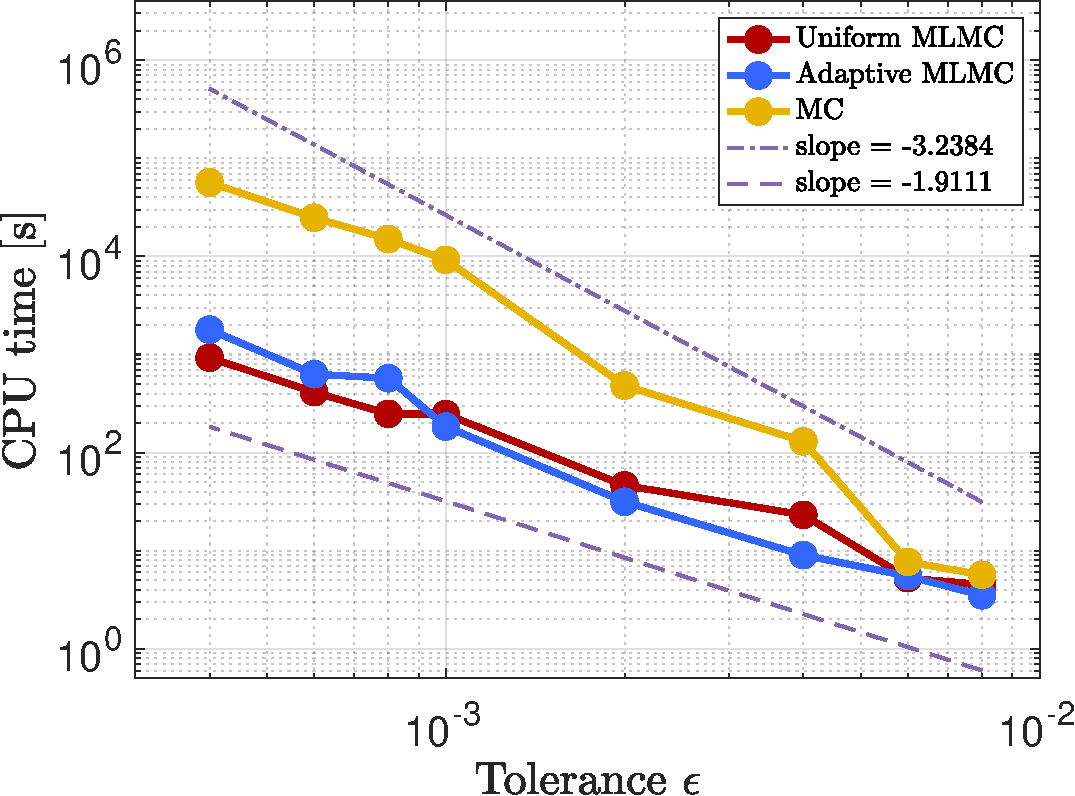
\includegraphics[height=0.35\linewidth]{CPUtime_epsilon_L2norm.pdf}&
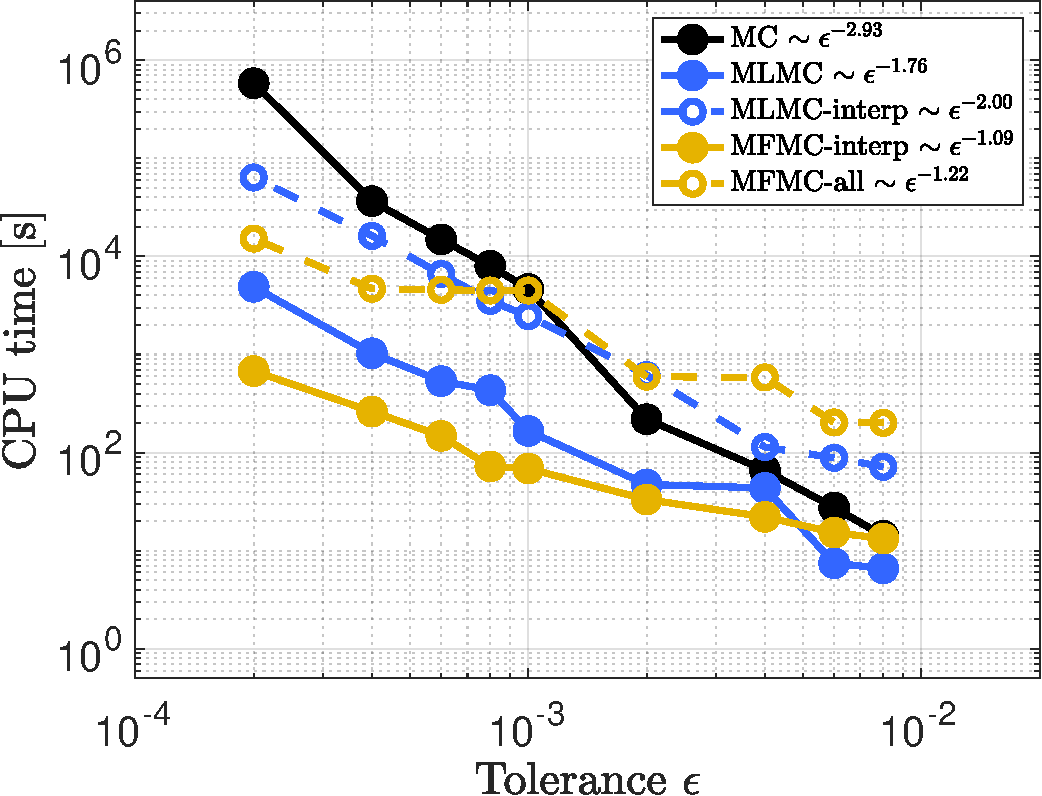
\includegraphics[height=0.4\linewidth]{./figures_slides/Cost_epsilon.pdf}
\end{tabular}
}
% \caption{Left: sampling cost (CPU time in seconds) of direct computation vs. tolerance $\epsilon$ for MC, MLMC with geometry-conforming uniform meshes, and MLMC with adaptive meshes.  Right: sampling cost vs. tolerance $\epsilon$ for MC with both direct computation and surrogate, MLMC with both direct computation and surrogate.} 
\label{fig:Experiment_result_plot}
\end{figure}

\end{itemize}
\end{frame}




%------------------------------------------------------------
\begin{frame}[t]
    \frametitle{Numerical results}

{\fontsize{7.8}{7.8}\selectfont 
\begin{theorem}[Asymptotic Cost for MFMC-SC Estimator]\label{thm:Sample_cost_est}
Consider a hierarchy of models $\{u_{\ell(k),k}\}_{k=1}^{K_c}$, where $u_{L,1}$ denotes the high-fidelity model on the finest mesh $\mathcal{T}_L$ with $M_L$ degrees of freedom, and the low-fidelity models $\{u_{\ell(k),k}\}_{k=2}^{K_c}$ are constructed via sparse grid stochastic collocation on coarser meshes $\mathcal{T}_{\ell(k)}$ with $\ell(k) = L + 1 - k$. Let $\mathcal{I} = \{i_k \mid k = 1, \dots, K\}$ denote the index set of selected models, ordered by decreasing correlation $\rho_{1,i_k}$ and associated costs $C_{i_k}$. For the family of high-fidelity models $\{u_{L,1}\}_{L\le L_{\max}}$ with $M_L$ degrees of freedom, assume  there exist positive constants $\alpha, \beta, \gamma$ such that
%
\begin{alignat*}{8}
    \text{(i)}\quad & \left\Vert \mathbb{E}[u] - \mathbb{E}[u_{L,1}] \right\Vert_U \simeq M_L^{-\alpha}, \qquad
    \text{(ii)}\quad & 1 - \rho_{1,i_2}^2 \simeq M_L^{-\beta}, \qquad
    \text{(iii)}\quad & C_1 \simeq M_L^{\gamma},
\end{alignat*}
%
For each low-fidelity model $u_{\ell(i_k),i_k}$ with $k = 2, \dots, K$, assume there exist positive constants $\beta_1, \gamma_1$ such that the correlation decay and cost growth follow
%
\begin{alignat*}{8}
    % &(i)\;\; |\rho_{1,1}|>\ldots>|\rho_{1,K}|,& \quad \quad
    % &(ii)\;\; \frac{C_{k-1}}{C_k}>\frac{\rho_{1,k-1}^2-\rho_{1,k}^2}{\rho_{1,k}^2-\rho_{1,k+1}^2},\;\;k=2,\ldots,K, \quad \rho_{1,K+1}=0,\\
    % &(iii)\;\; 1-\rho_{1,i_2}^2 \simeq M_{L}^{-\beta},
    % \qquad
    &(iv)\quad \rho_{1,i_k}^2-\rho_{1,i_{k+1}}^2 \simeq M_{\ell(i_k)}^{-\beta_1},
    \qquad
&(v)\quad C_{i_k} \simeq M_{\ell(i_k)}^{\gamma_1},
\end{alignat*}
%
with $\rho_{1,i_{K^*+1}}^2 := 0$. Then, for any tolerance $\epsilon \in (0, e^{-1})$, there exists a finest mesh level $L \le L_{\max}$ and sample allocation $\{N_{i_k}\}_{i_k \in \mathcal{I}^*}$ such that the multifidelity estimator $A^{\mathrm{MF}}$ achieves an bounded nMSE  with $\epsilon^2$. In the regime where the high-fidelity contribution dominates, the total cost reduces to
%
\[
\mathcal{W}^{\mathrm{MF}} \lesssim \epsilon^{-2 - \frac{\gamma-\beta}{\alpha}}.
\]
%
\end{theorem}
}
\end{frame}







%------------------------------------------------------------
\begin{frame}[t]
    \frametitle{Numerical results}
\begin{itemize}[leftmargin=5pt] 
% \item[$\triangleright$] \textcolor{myblue3}{\bf Surrogate-enhanced multilevel Monte Carlo:} {\footnotesize Integrate surrogate with multilevel Monte Carlo.}
\item[$\triangleright$] \textcolor{myblue3}{\bf Accuracy:} 
{\footnotesize Plasma boundary and geometric descriptors from MFMC sampling exhibit behavior consistent with those from MC and MLMC when interpolated onto a common mesh.}
% \item[$\triangleright$] \textcolor{myblue3}{\bf Efficiency:} {\footnotesize 
%  Su.}
%  \vspace{3mm}
\begin{figure}[ht!]\centering
\scalebox{0.19}{
\begin{tabular}{cccc}
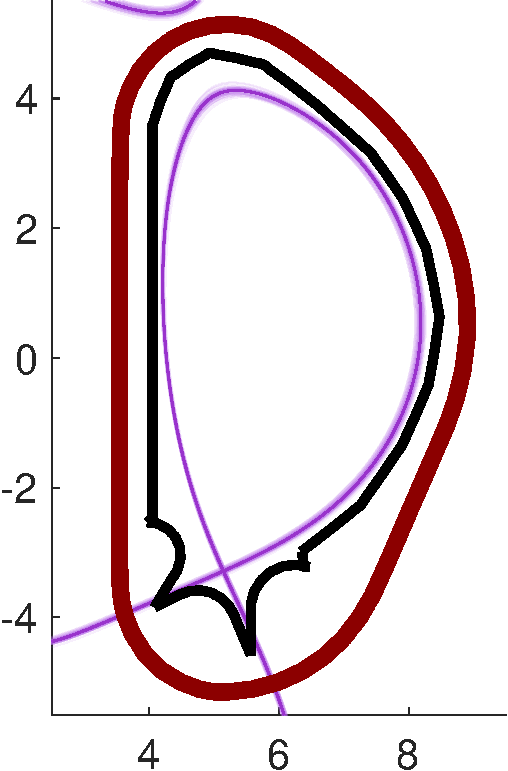
\includegraphics[width=1\linewidth]{./figures_slides/QoI_MC_uniform.pdf}
&\includegraphics[width=1\linewidth]{./figures_slides/QoI_MLMC_DirectSolver_Interp2CommonGrid.pdf}
&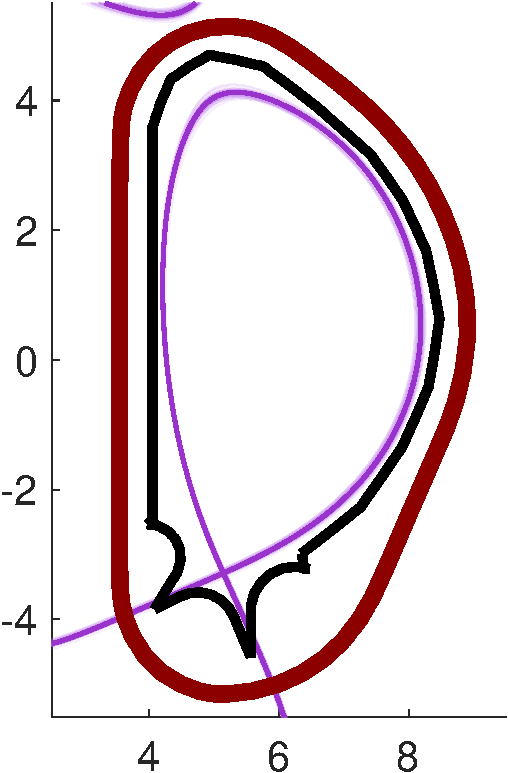
\includegraphics[width=1\linewidth]{./figures_slides/QoI_MFMC.pdf} 
% &\includegraphics[width=1\linewidth]{QoI_MLMC_surrogate.pdf} 
% &\includegraphics[width=1\linewidth]{QoI_MLMC_DirectSolver_Interp2CommonGrid.pdf} 
% &\includegraphics[width=1\linewidth]{QoI_MLMC_surrogate_Interp2CommonGrid.pdf} 
\\
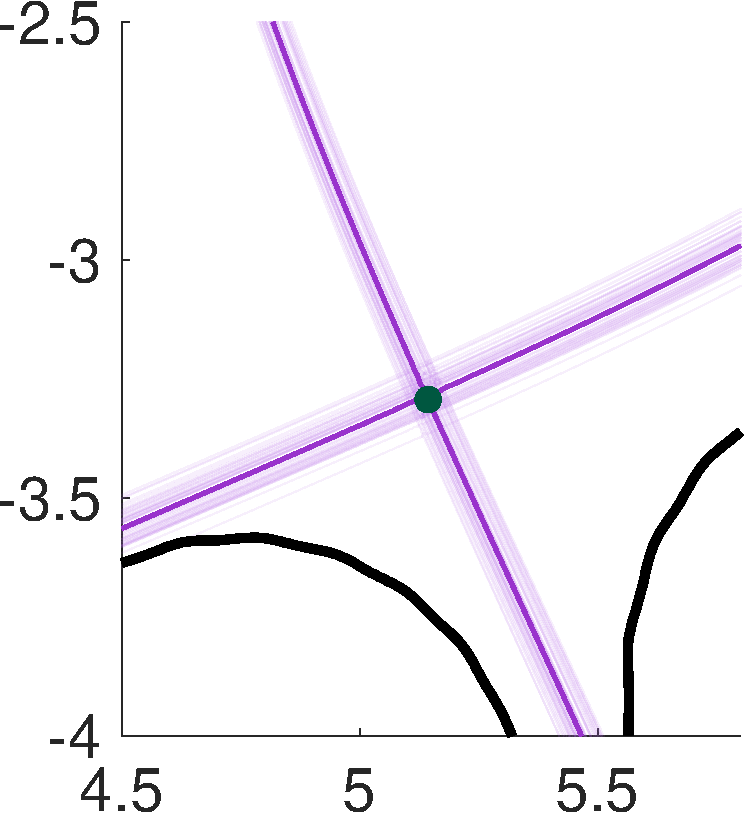
\includegraphics[width=1\linewidth]{./figures_slides/QoI_MC_uniform_xptRegion.pdf} 
&\includegraphics[width=1\linewidth]{./figures_slides/QoI_MLMC_DirectSolver_xptRegion_Interp2CommonGrid.pdf} 
&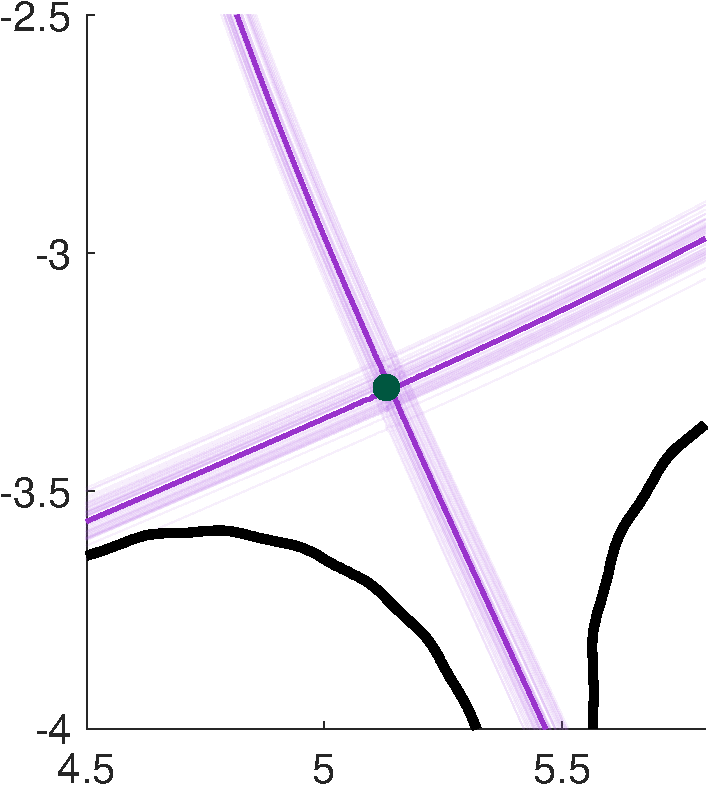
\includegraphics[width=1\linewidth]{./figures_slides/QoI_MFMC_xptRegion.pdf} 
% &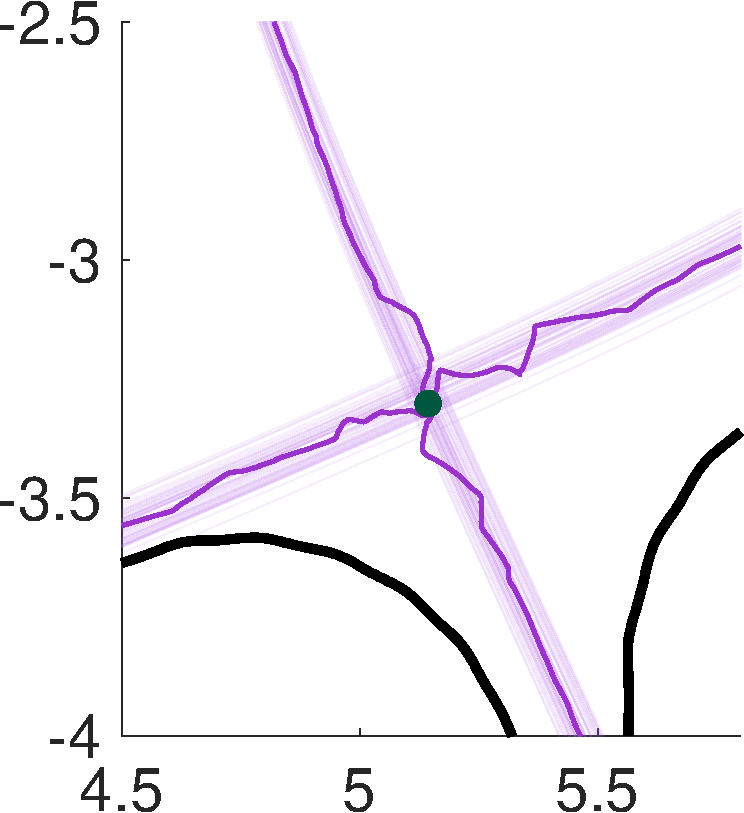
\includegraphics[width=1\linewidth]{QoI_MLMC_surrogate_xptRegion.pdf} 
% &\includegraphics[width=1\linewidth]{QoI_MLMC_DirectSolver_xptRegion_Interp2CommonGrid.pdf}
% &\includegraphics[width=1\linewidth]{QoI_MLMC_surrogate_xptRegion_Interp2CommonGrid.pdf}
\\[1ex]
\quad {\fontsize{35}{35}\selectfont MC-FE} & {\fontsize{35}{35}\selectfont MLMC-FE (Interp)}  &{\fontsize{35}{35}\selectfont MFMC-FE (Interp)}
% & {\fontsize{35}{35}\selectfont MLMC + Direct + interp} 
% &{\fontsize{35}{35}\selectfont MLMC + Surrogate + interp} 
\\[-0.5ex]
\end{tabular}
}
\end{figure}


%
% \vspace{1mm}
% \item[$\triangleright$] {\bf This project is in preparation.}
% \vspace{1mm}
        
% {\fontsize{8}{8}\selectfont \textcolor{mygray2}{In preparation.}
% \par}
\end{itemize}
\end{frame}







%-----------------------------------------------------------
\begin{frame}
% \frametitle{$|\!\!\sim\! \underline{\hspace{0.25cm}}\!\sim\!\! |@ \underline{\hspace{0.25cm}} @|\!* \!\underline{\hspace{0.25cm}}\!*\!|. \underline{\hspace{0.25cm}} .|- \underline{\hspace{0.25cm}} -|G \underline{\hspace{0.25cm}} G|x\underline{\hspace{0.25cm}} x|/\underline{\hspace{0.25cm}}\backslash|w_w|Q\underline{\hspace{0.25cm}}Q|>\underline{\hspace{0.25cm}}>|=\underline{\hspace{0.25cm}}=|+\underline{\hspace{0.25cm}}+|\#\underline{\hspace{0.25cm}}\#|z\underline{\hspace{0.25cm}}z|>\underline{\hspace{0.25cm}}<|6\underline{\hspace{0.25cm}}9|$}


	\begin{center}
	{\fontsize{35}{70}\selectfont  Thank You $|\neg\underline{\hspace{0.4cm}}\neg|$}
	\end{center}
\end{frame}
%----------------------------------------------------------------
\end{document}